%\documentclass[a4paper, 11pt]{article}
\documentclass[fleqn,10pt]{olplainarticle}
\usepackage{comment} % enables the use of multi-line comments (\ifx \fi) 
% \usepackage{fullpage} % changes the margin
% \usepackage{graphicx}
% \usepackage{tabu}
% \usepackage{array}
% \usepackage{booktabs}
% \usepackage{hyperref} 
% \usepackage{color}
% \usepackage{mathtools}
% \usepackage[utf8]{inputenc}
% \usepackage{enumitem}
% \usepackage{amssymb}
% \usepackage{soul}
% \usepackage{graphicx} 
% \usepackage{amsmath, amsthm, amsfonts, amssymb, amscd, bm}
% \usepackage{verbatim}
% \usepackage{url}
\usepackage{tabularx}
% \usepackage{xspace}
% \usepackage[square,numbers]{natbib}
% \usepackage{lineno}
\usepackage{multirow}
\usepackage{longtable}

\usepackage{draftwatermark}
\SetWatermarkText{DRAFT}
\SetWatermarkScale{1}


\usepackage{soul}
\PassOptionsToPackage{hyphens}{url}\usepackage{hyperref}

% \usepackage{tgadventor}
% \renewcommand*\familydefault{\sfdefault} %% Only if the base font of the document is to be sans serif
% \usepackage[T1]{fontenc}

\usepackage[skip=0.5\baselineskip]{caption}
\usepackage{subcaption}


\title{Indices of Human-Wildlife Conflict.}

\author[1,2]{G.E. Ryan}

\affil[1]{Telethon Kids Institute, Nedlands, WA, Australia}
\affil[2]{Centre for Epidemiology and Biostatistics, Melbourne School of Population and Global Health, The University of Melbourne, VIC, Australia}

keywords{human-wildlife conflict, elephant, tiger, monitoring, ecological indices, conservation}
\cfoot{This is a draft and has not yet been peer reviewed or published}

\begin{document}
\flushbottom
\maketitle
\noindent\normalsize 
%\begin{figure}[!ht]
%    \centering
%    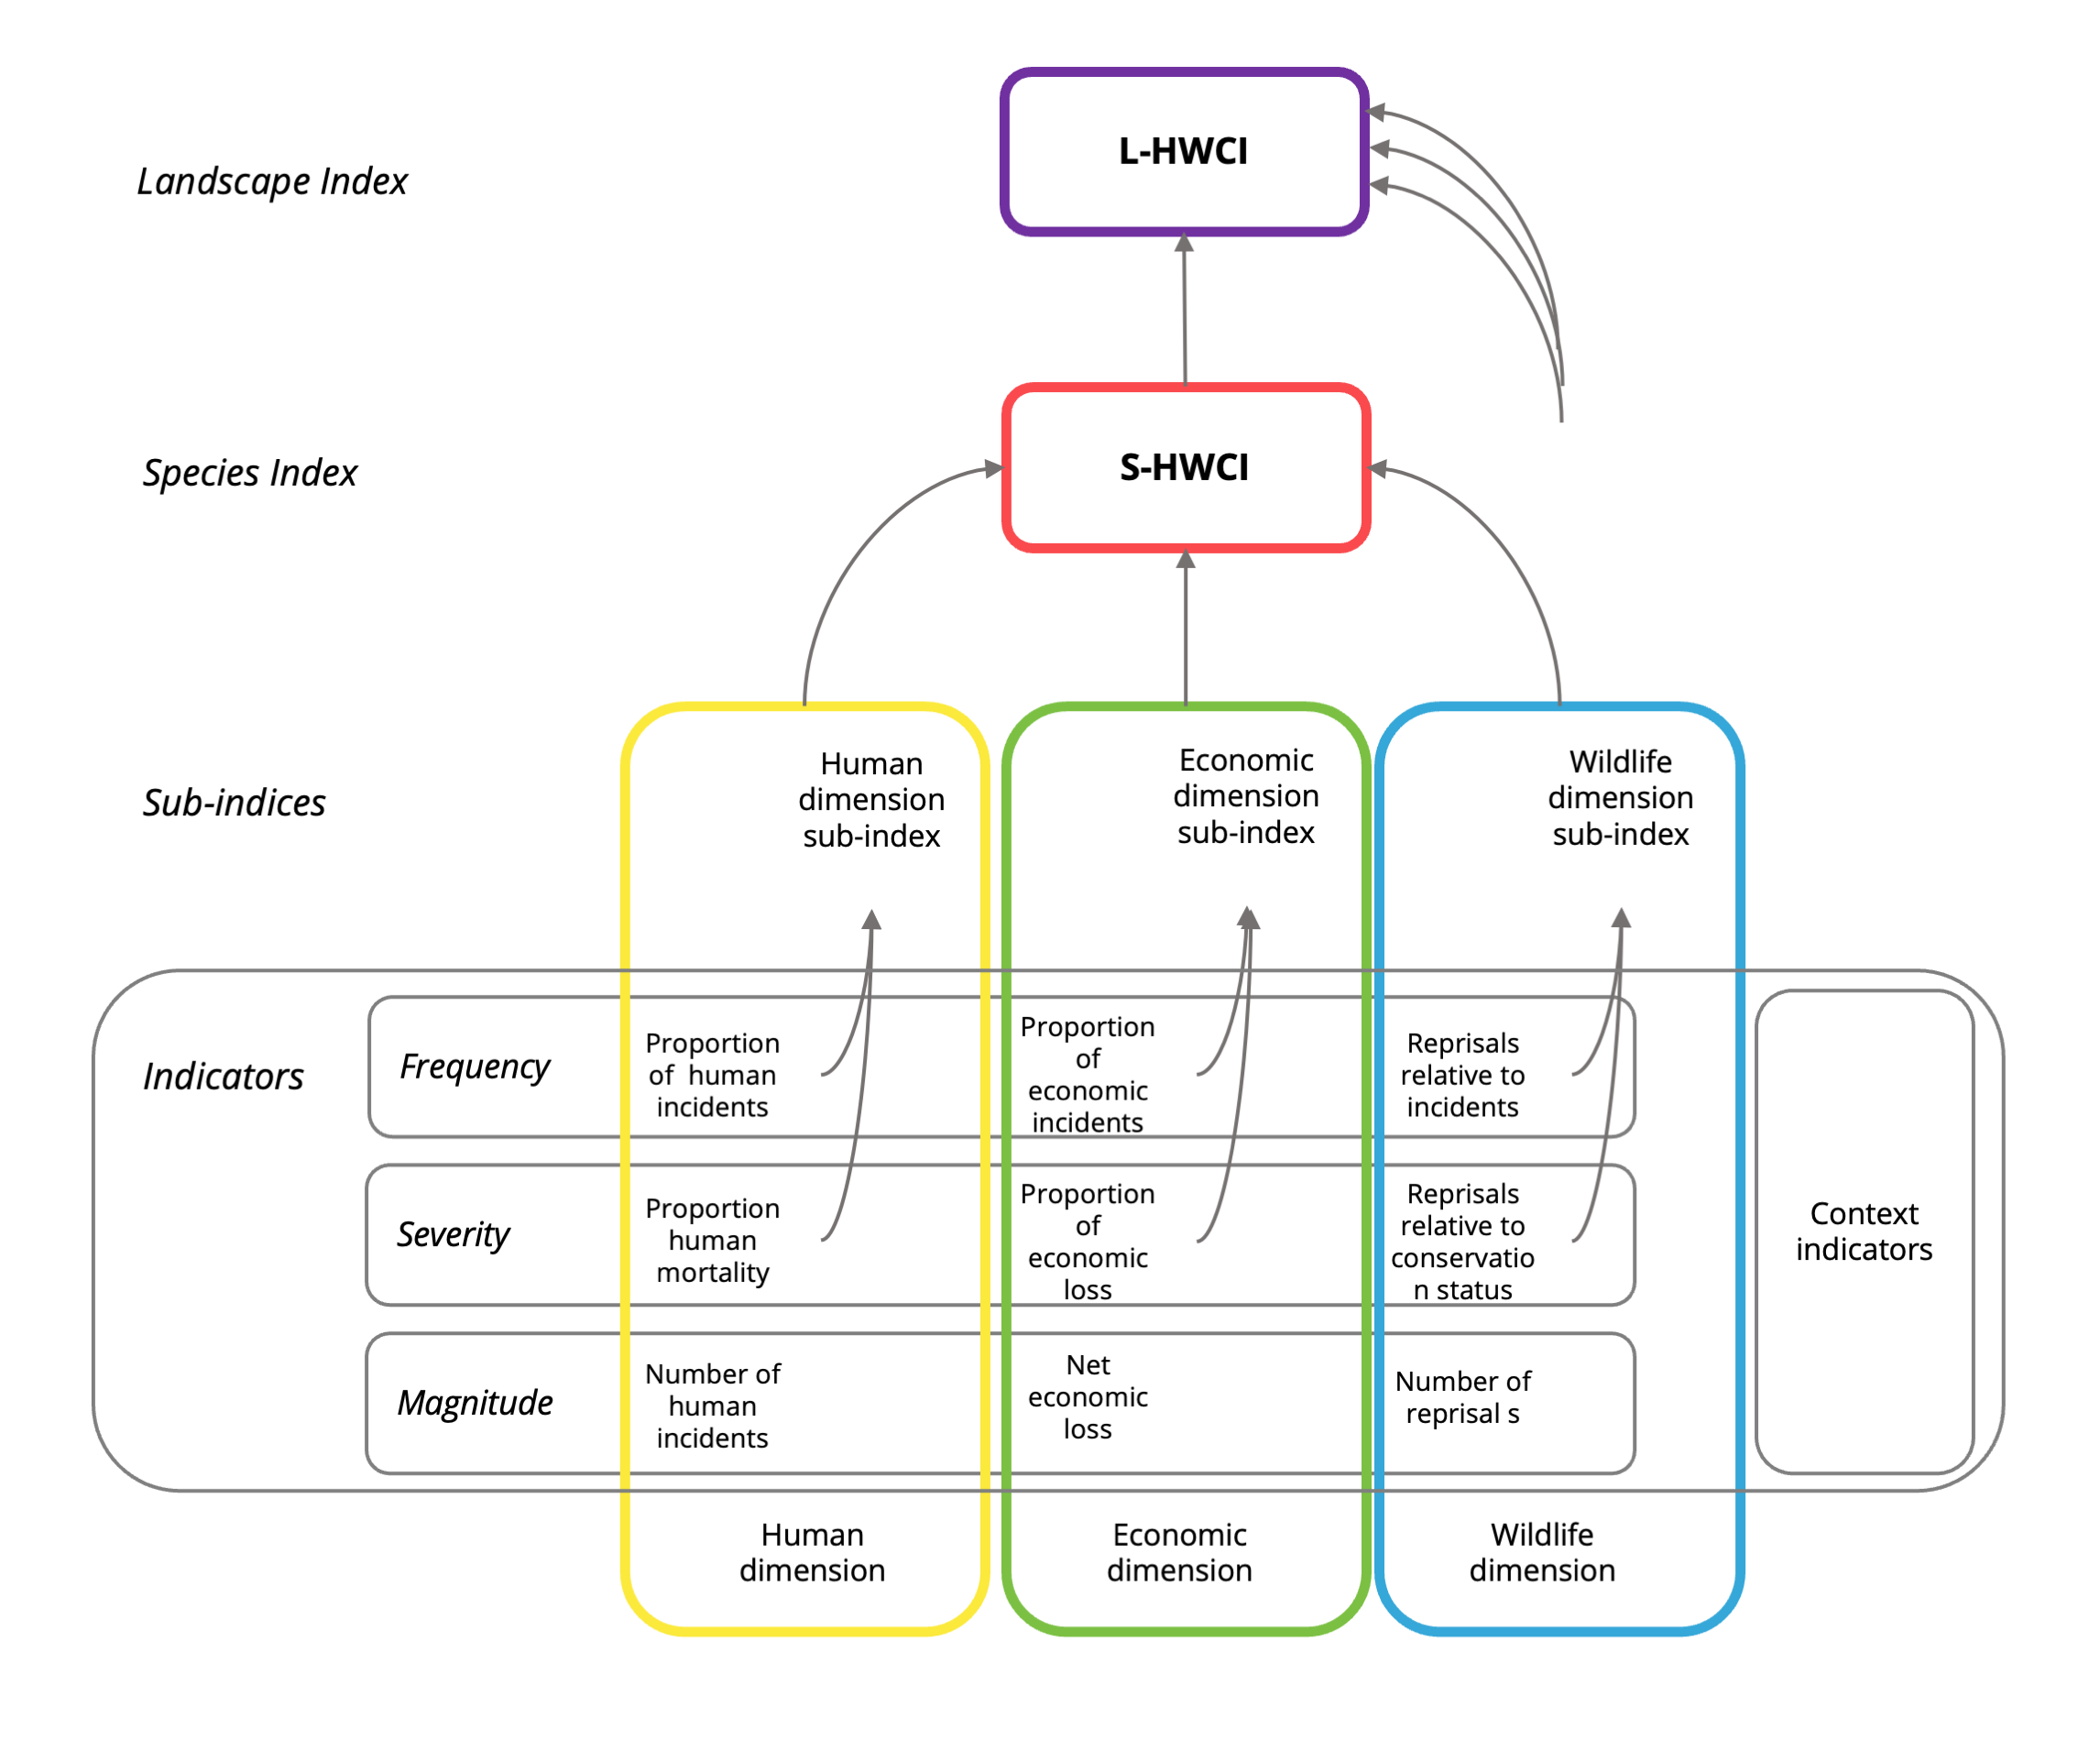
\includegraphics[width = 1\textwidth]{hwci_hierarchical_diagram_20221117.png}
%    \caption{The hierarchical framework of the proposed index of human-wildlife conflict.}
%    \label{fig:framework}
%\end{figure}
\section*{Summary}
\textbf{Key points:}
\begin{itemize}
    \item This summary document describes a composite index of human-wildlife conflict (HWC) inteneded to track HWC in landscapes over time.
    \item The index consists of a top-level index for a species, which sits over three sub-indices for the human, economic, and wildlife dimensions of the problem. Each sub-index is calculated from indicators of the frequency and severity of HWC in each dimension. Species-level indicators can be combined for multi-species landscale indices.
    \item The indices and indicators are scaleable and directly comparable among landscapes, and can be appied at any level from the village or park, to nations or continents.
    \item The index uses from fundamental HWC and demographic data, but is able to use richer data if available. 
    \item The basic data needed are:
    \begin{itemize}
        \item Number of households in the landscape (or average household size  and landscape population) 
         \item Number of human-victim incidents  
         \item Number of human mortalities 
         \item Number of economic incidents in the landscape 
         \item Economic losses in the landscape 
         \item Mean economic wealth of households in the landscape 
         \item Number of wildlife-victim incidents in the landscape 
         \item Target species' IUCN Red List status 
    \end{itemize}
    \item The index cannot directly overcome under-reporting of HWC, as would any simpler summary or count of incidents.
\end{itemize}

Here we develop an index of human-wildlife conflict as a mechanism to summarise information about a complex and multifaceted problem. The aims of the mechanism are to enable immediate understanding of the relative state of HWC in different landscapes, to be applicable and comparable over different geographic scales, to be easy to communicate, and to retain key detail while simplifying a complex situation. We also explore lessons from a range of global indices, and the potential for the application of index-based insurance to HWC.
The index developed consists at the base level of a range of indicators representing the frequency, severity, and magnitude of HWC incidents in a landscape. These indicators are split among three different dimensions of the problem: the human dimension, i.e., direct effects of HWC on humans such as injuries and deaths; the economic dimension, i.e., the economic effects of HWC such as damage to crops, killing of livestock, or damage to equipment; and the context dimension, which represents the context in which HWC occurs and includes the impacts to wildlife through reprisals for HWC, the attitudes of the local community to wildlife, and a range of other indicators specific to the local landscape context. Indicators are combined to calculate sub-indices for each of the three dimensions, and the sub-indices are combined to calculate the headline index of human-wildlife conflict. It is intended that the index is displayed in conjunction with sub-indices and indicators so that while the index can display simply the overall situation, by glancing down at indicators, one is able to ascertain sources of variation and nuance. Thus we hope to get the benefit of a simple overall index, whilst retaining the much of the important detail that provides context to interpret this index in the indicators below.
We explore this index of human-wildlife conflict by testing its performance in a simulated landscape and apply it to real data from Nepal. Results from the simulations suggest that the index behaves as expected. Application to Nepal demonstrates that the index can be immediately applied to real data, however also demonstrate the limitations in dealing with uncertainty and missing data. These are key knowledge gaps to fill in future development of the index. Robust and systematic collection of HWC data will also be key to applying the index in future. Overall the index of human-wildlife conflict developed here shows great promise as a mechanism to summarise and compare HWC.


\section*{Introduction}

This summary report describes an in-development index of human-wildlife conflict.  Human-wildlife conflict (HWC) is a global social and environmental problem and is extremely complex. HWC involves species as varied as geese, sharks, kangaroos, and elephants, and the direct results range from negligible damage to domestic gardens, to losses of livelihoods, homes, and lives. The flow-on effects of human-wildlife conflict can sour the community attitudes to local wildlife, resulting in in the persecution of perceived perpetrator species, undermine support for environmental protection measures, and can stress people and livestock which reduces productivity and quality of life. While historically much effort focused on actions to prevent HWC and mitigate its impacts, new work is now being done to understand and manage the problem from diverse perspectives. This is where an index of human-wildlife conflict can help.

One framing of management of human wildlife conflict is through six key elements: understanding the conflict, policy, prevention, response, mitigation, and monitoring. An index can potentially help with a number of these elements. The scale and intensity of human wildlife conflict is generally poorly understood and inconsistently measured. An index could be useful for comparing like-for-like among countries and regions, and at a range of different scales. Such an index could be useful to highlight problem areas or areas where conflicts are being well managed. An index could also be useful as a monitoring tool, to assess progress in HWC management over time. The types of conflicts and underlying causes can differ widely. For instance conflicts may be heightened at intermediate levels of habitat or human density, with lower levels of conflict at the extremes of high levels of habitat or high levels of human density (Brooks n.d.). A suitable index may be able to help easily differentiate these conflict types. 

Here we briefly describe a plausible and practical index and show an example from simulated data, and from real HWC data from Nepal from 2006–2016. The index requires only minimal data; namely records of HWC, simple demographic data, and the IUCN Red List status of target species \ref{tab:min_data}.


\begin{table}[!h]
    \centering
    \caption{Minimum data required to calculate Species Human Wildlife Conflict Index}
    \label{tab:min_data}
    \begin{tabular}{>{\raggedright\arraybackslash}p{13cm}}
         Number of households in the landscape (or average household size  and landscape population) \\
         Number of human-victim incidents  \\
         Number of human mortalities \\
         Number of economic incidents in the landscape \\
         Economic losses in the landscape \\
         Mean economic wealth of households in the landscape \\
         Number of wildlife-victim incidents in the landscape \\
         Target species' IUCN Red List status \\
          
    \end{tabular}
\end{table}


The key aims for an index of human-wildlife conflict are to:
\begin{itemize}
    \item Rapidly identify the HWC status of a given area
    \item Be scaleable, and so applicable at scales from local to global
    \item Be useful as a monitoring tool
	\item Illuminate conflict types
    \item Be a useful communications tool
    \item Cope with missing data.
\end{itemize}


\section*{Index design}

\subsection*{Theoretical framework}
We hope to develop an index that allows us to quickly understand the status of HWC occurring in an area, different types of conflict, and is scaleable and useful for monitoring, and communication. To fulfil the aim of simplicity and facilitate rapid understanding of a situation requires synthesis of a complex array of information. This conflicts with the ability to easily understand different types of conflict and the many elements of HWC that may not move in the same direction at once. To this purpose we propose a single composite index to describe the overall situation, composed of a series of sub-indices and indicators that allow for a more nuanced and detailed understanding of the underlying situation.

\begin{figure}[!ht]
    \centering
    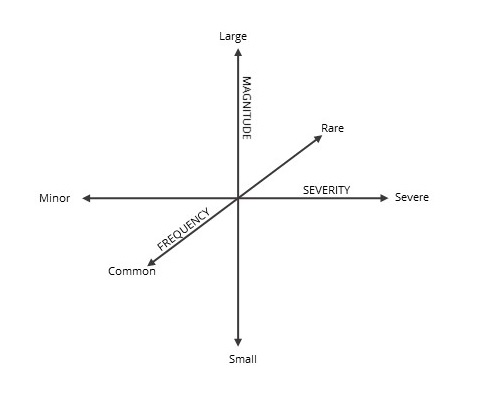
\includegraphics[width = 1\textwidth]{axes.jpg}
    \caption{Indicators of HWC impact: severity, frequency, and magnitude. Adapted from Nyhus (2016).}
    \label{fig:indicators}
\end{figure}

\subsection*{Dimensions of conflict}
Here we consider ‘dimensions’ of HWC as broad differing components of HWC that represent very distinct types of HWC or components of HWC. Noting that we are interested in HWC in the sense of the impact of wildlife on humans and human activity, rather than e.g. conflict among humans over wildlife. The impacts of wildlife on humans are complex and varied, however we consider two broad ‘dimensions’ that we are terming the ‘human dimension’ and the ‘economic dimension’:
The human dimension includes direct impacts on human life, which includes direct harm such as injuries and death, as well as psychological of other health impacts.
The ‘economic dimension’ includes  indirect impacts on humans such as the loss of crops or livestock, damage to homes, fencing, or other structures, raiding food storage, etc.
The rationale for making this distinction is because it avoids making assumptions about values. While it may be possible to attribute some economic value to injuries or human lives using a range of methods, these are ultimately contestable and based on the values of those assigning them, and will vary with location and social context. Moreover, aside from the necessity of achieving agreement on relative values, there is a value judgement in comparing impacts to human live with impacts to property at all. We therefore believe it is important to maintain this distinction between areas of impact.
 To understand HWC more broadly we must also consider these impacts against the context in which they occur. Here we consider this the ‘context dimension’:
The context dimension includes information about the social context of HWC such as community attitudes toward wildlife, and responses to HWC, and information about the status of wildlife species.
For example, are people positive and tolerant to wildlife, or negative and afraid? Are there reprisals against wildlife in response to HWC? Are wildlife populations abundance or rare? Rising or declining? Is the landscape patchy, human dominated, and with little remaining habitat, or dominated by barely disturbed wilderness and few people? All of these dimensions present important parts of the understanding the type of HWC and provide very different information to decision makers.

\begin{figure}
    \centering
    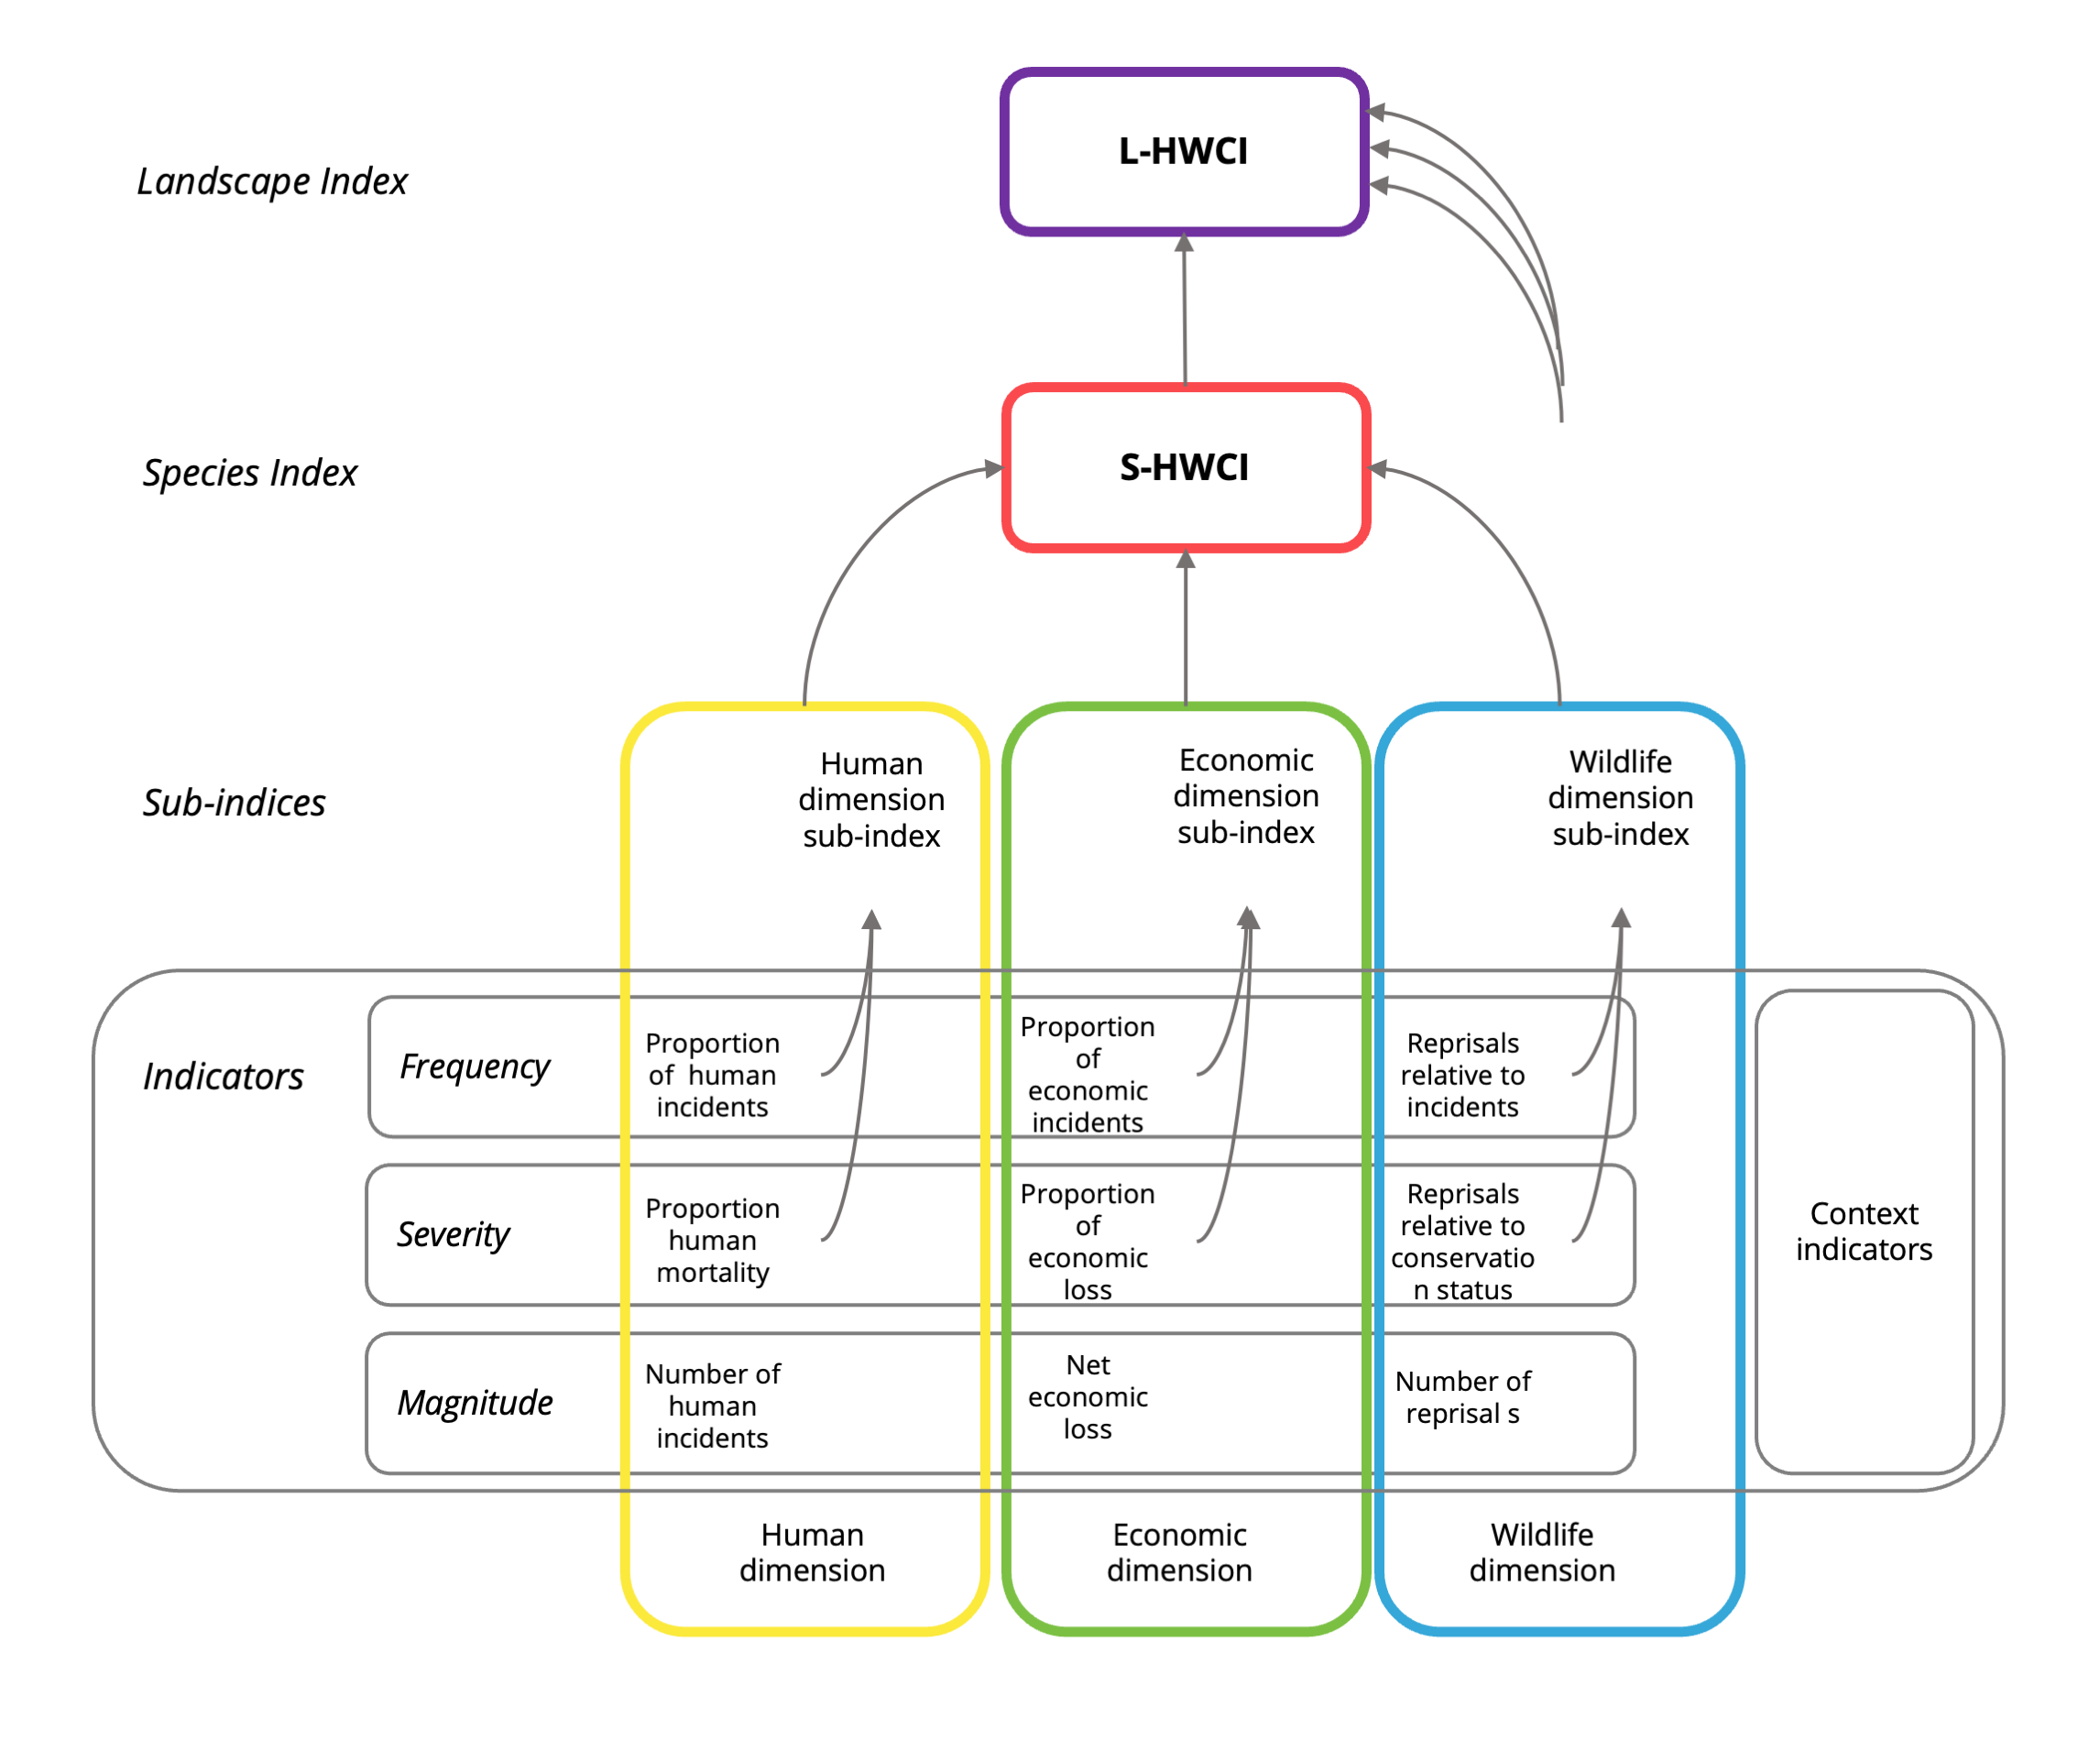
\includegraphics[width = 1\textwidth]{hwci_hierarchical_diagram_20221117.png}
    \caption{The hierarchical framework of the proposed index of human-wildlife conflict.}
    \label{fig:framework}
\end{figure}

\subsection*{Indicators of impact}
Within a single dimension, impacts from HWC can occur on a continuum of other measures. Nyhus (2016) presents a framework where interactions between wildlife and people occur in three axes where the type of interaction ranges from negative to positive, the frequency from rare to common, and the ‘impact’ from minor to severe. Here we modify this concept. Given that we are interested in conflicts, we exclude positive interactions, and consider that the scale of negativity is likely to be driven by the severity and frequency. Therefore we ignore this positive-negative scale for this purpose, and re-imagine these axes as indicators representing increasing aggregations of the problem \ref{fig:indicators}.
A single incident may occur on a continuum of severity from minor incidents like seagulls pestering beach-goers for scraps, to severe incidents like loss of human life. On aggregate, incidents affecting an individual or household, may occur on a continuum of frequency from rare, e.g. unlikely in a lifetime, to frequent, e.g. a daily occurrence. And on further aggregate across a landscape, incidents which may be severe or not, and frequent or not, may sum to a large total, or a much smaller one, for instance frequent and severe predator attacks on livestock in a single small town may be a very important local landscape problem, but a relatively smaller one at the scale of a country of tens of millions of people, while crop damage may be relatively minor locally, but if occurring nationwide may be considered of much greater magnitude.
By examining impacts along each of these indicators, we are able to understand important distinctions in the form of HWC. 

 
\subsection*{Index structure}
Here we propose a hierarchical index of HWC, which is outlined in Figure 3. At the base level are indicators. For each dimension, there are indicators of HWC severity, frequency, and magnitude. At the next level, there is a sub-index for each dimension. The sub-indices composed of the severity and frequency indicators for that dimension. At the top level is the index, which is calculated from the three sub-indices. Together we refer to this collection as the suite of indicators. The suit of indicators can be calculated for a species, and species-level indices can be combined to form landscap-level indices.
The rationale for this structure is that at the top level, the index provides a simple measure of the status of HWC at either a landscape or species level. Below the this the dimension sub-indices provide a picture of these different areas of conflict, and below this the indicators provide a more detailed understanding of the patterns of HWC that underlie the index. It is intended that where possible, the index is used and displayed along-side the suite of sub-indices and indicators to provide an immediate overall as well as more detailed view of HWC. Each of the indicators is intended to be easy to understand, easy to calculate, and yet to provide useful insight into one aspect of human-wildlife conflict in a target landscape. Each indicator only able to represent one specific source of information, and together they do not represent every element of the conflict. However the aim is that the suite of indicators can together represent a detailed and nuanced description of HWC, allowing managers to quickly differentiate different sorts of HWC issues, while summarising a large amount of complex information in a simple format. Naturally more detailed analyses are not precluded and may provide other information about HWC that is not provided by this hierarchical index. 
Details of the construction of these indices and indicators within the hierarchical index are outlined in the following section “Index formulation”. The index components are listed in Table 2.

\section*{Index application}

\subsection*{Simulated examples}
This is a simulated example with three simulated species types:
species 1 is a large-carnivore type, Critically Endangered, with no economic impact, but human-victim incidents including mortalities, and subsequent reprisal killings of wildlife. Species 2 is a crop-pest type, Least Concern, with economic impacts but no human-victim incidents and few reprisals. Species 3 is an elephant type, Endangered, with impacts on human victims, economic damage, but no reprisal killings. Each species is simulated over 100 years with randomly generated data around some mean that is either stable or increasing over time.

\subsubsection*{Species 1}
For species 1 we see flat indicators for the economic-dimension, as expected with no economic damage. We see worsening indicators for the human-dimension frequency and magnitude, and stable though highly varied severity \ref{fig:sp1}. The wildlife-dimension severity indicator pivots between 1 and 0, as a result of being CR, the indicator value is zero when individuals are killed and 1 when no reprisals occur. These values reflect in the sub-indices, with slight declines in the human-dimension sub-index, and a usually low wildlife-dimension sub-index that fluctuates 

\begin{figure}
    \centering
    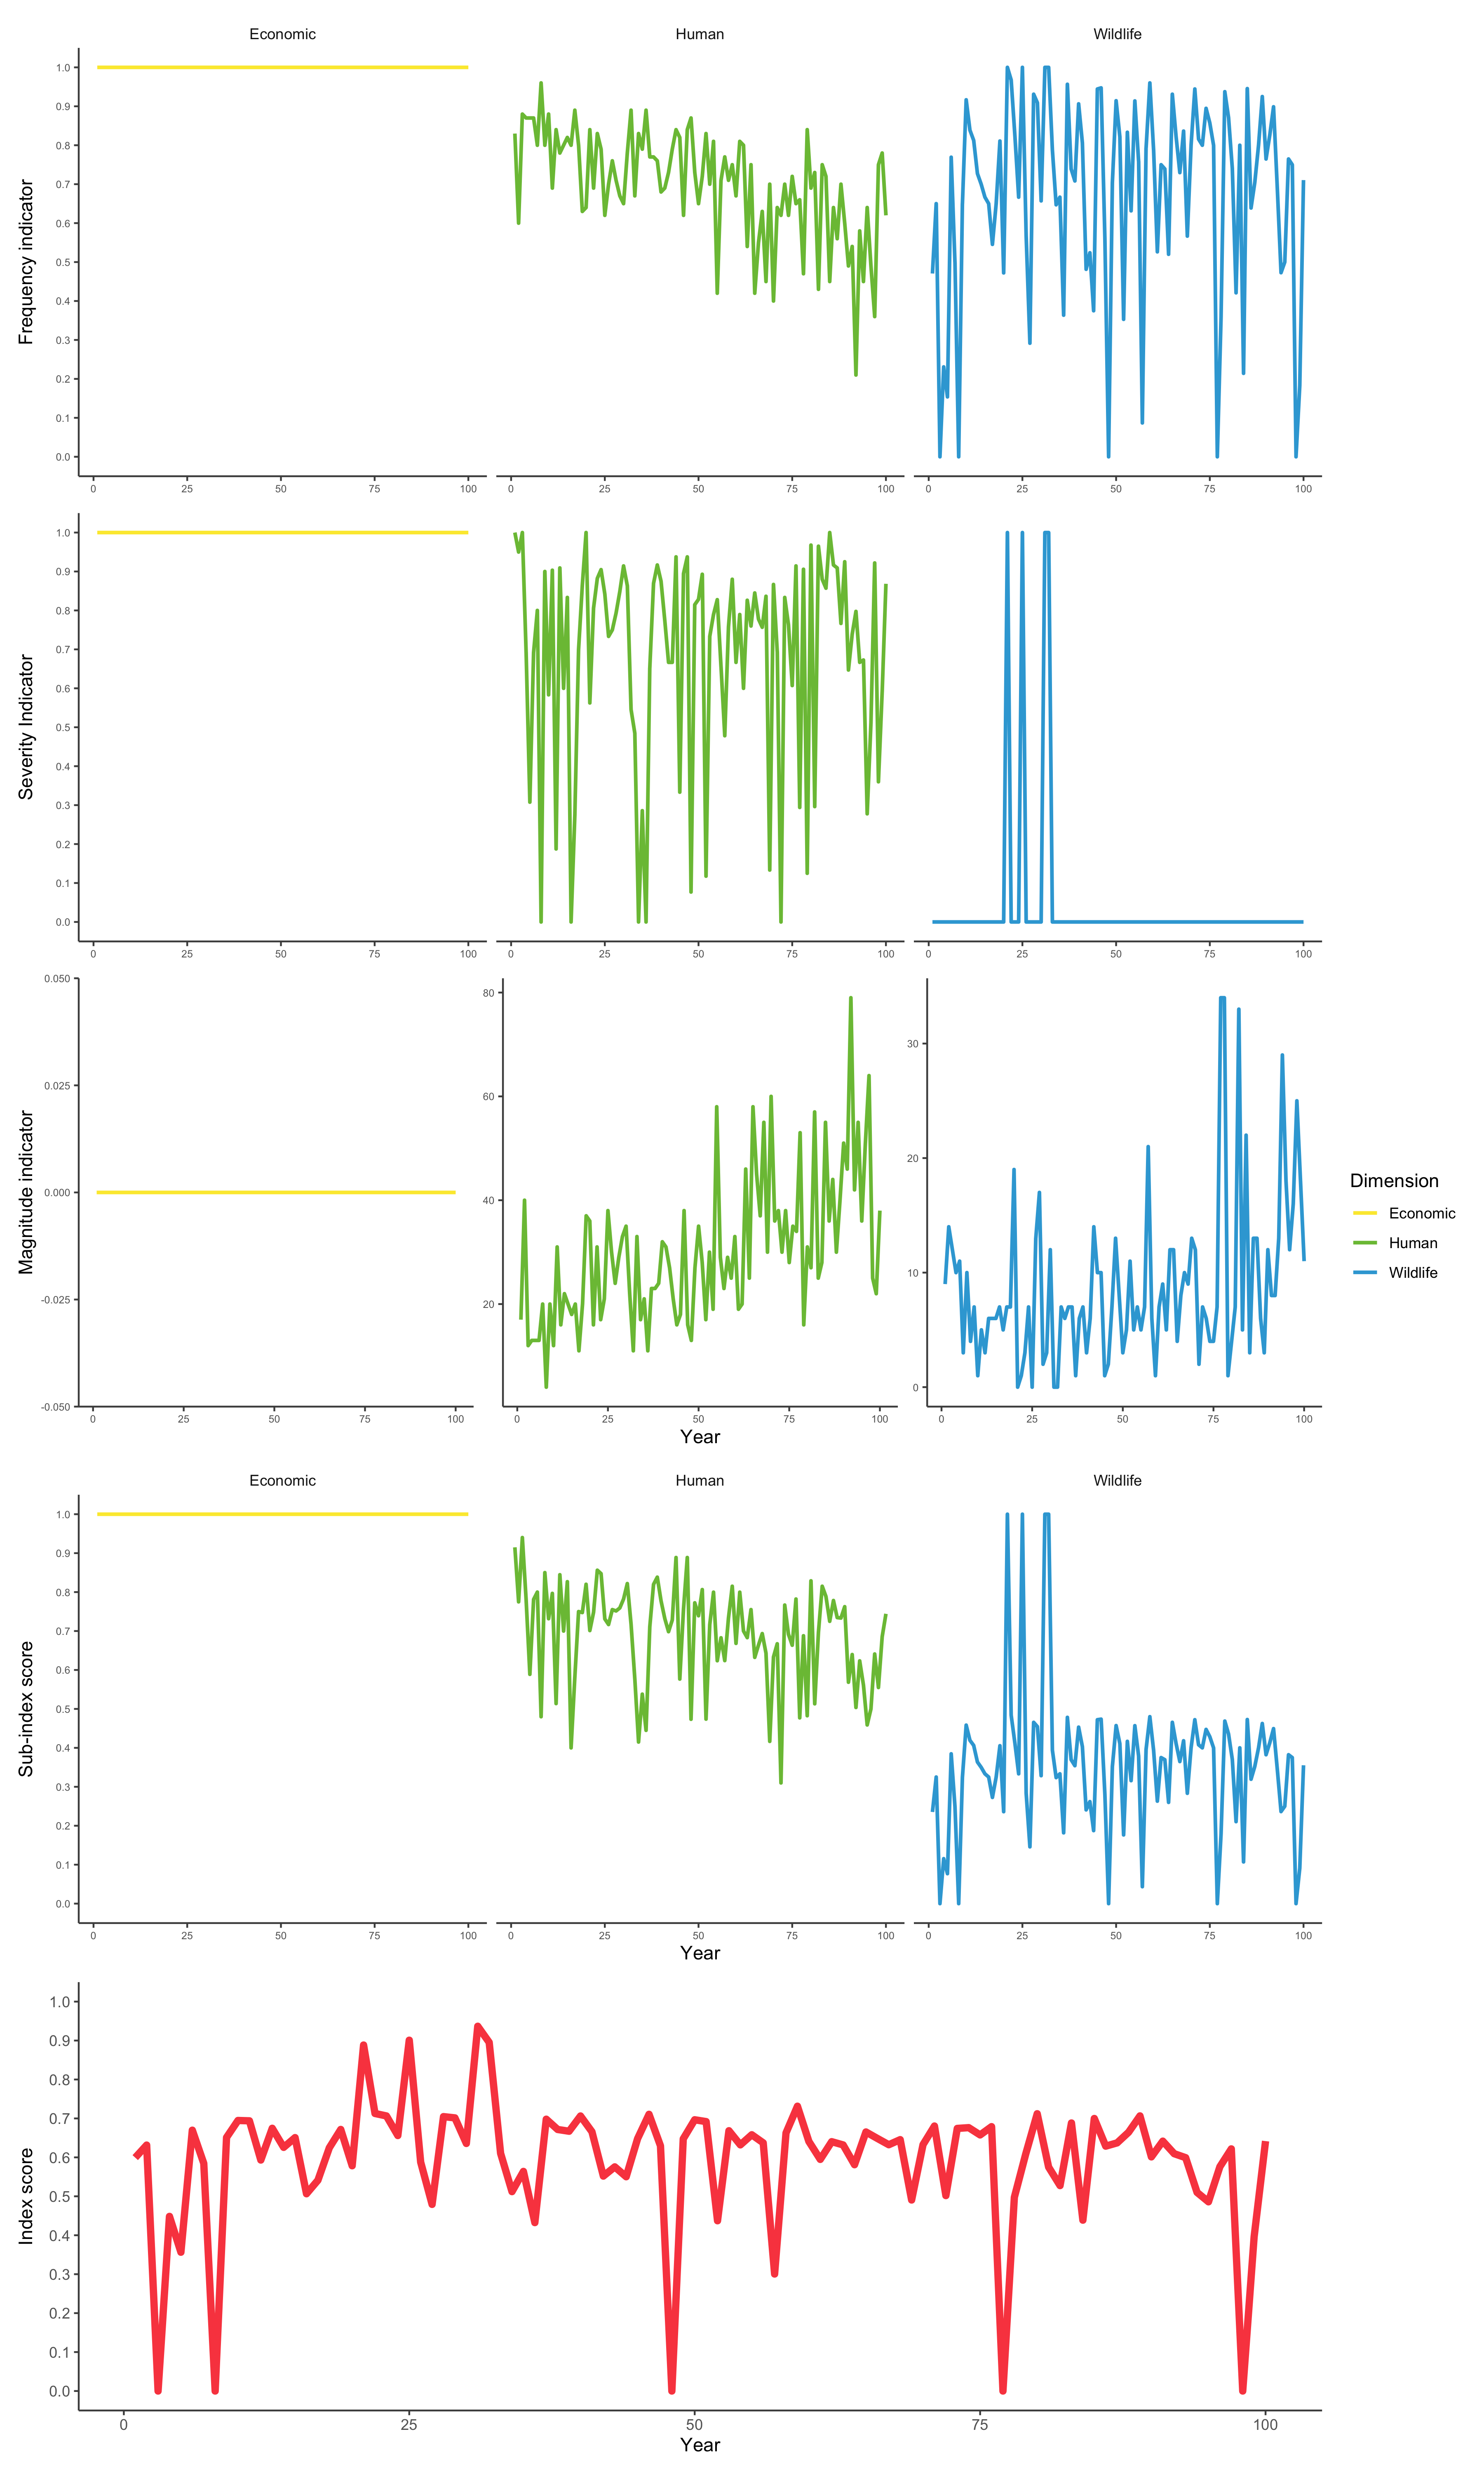
\includegraphics[width = 1\textwidth]
    {sp1_all.png}
    \caption{Indicators, sub-indices, and index of human-wildlife conflict for simulated Species 1}
    \label{fig:sp1}
\end{figure}

\subsubsection*{Species 2}
Species 2 performs as expected --- flat indicators and sub-indices for the human- and wildlife-  dimensions, and small decline in the economic-dimension frequency indicator \ref{fig:sp2}. This results in an overall high but very slowly declining species-level index of human-wildlife conflict \ref{fig:sp2}.

\begin{figure}
    \centering
    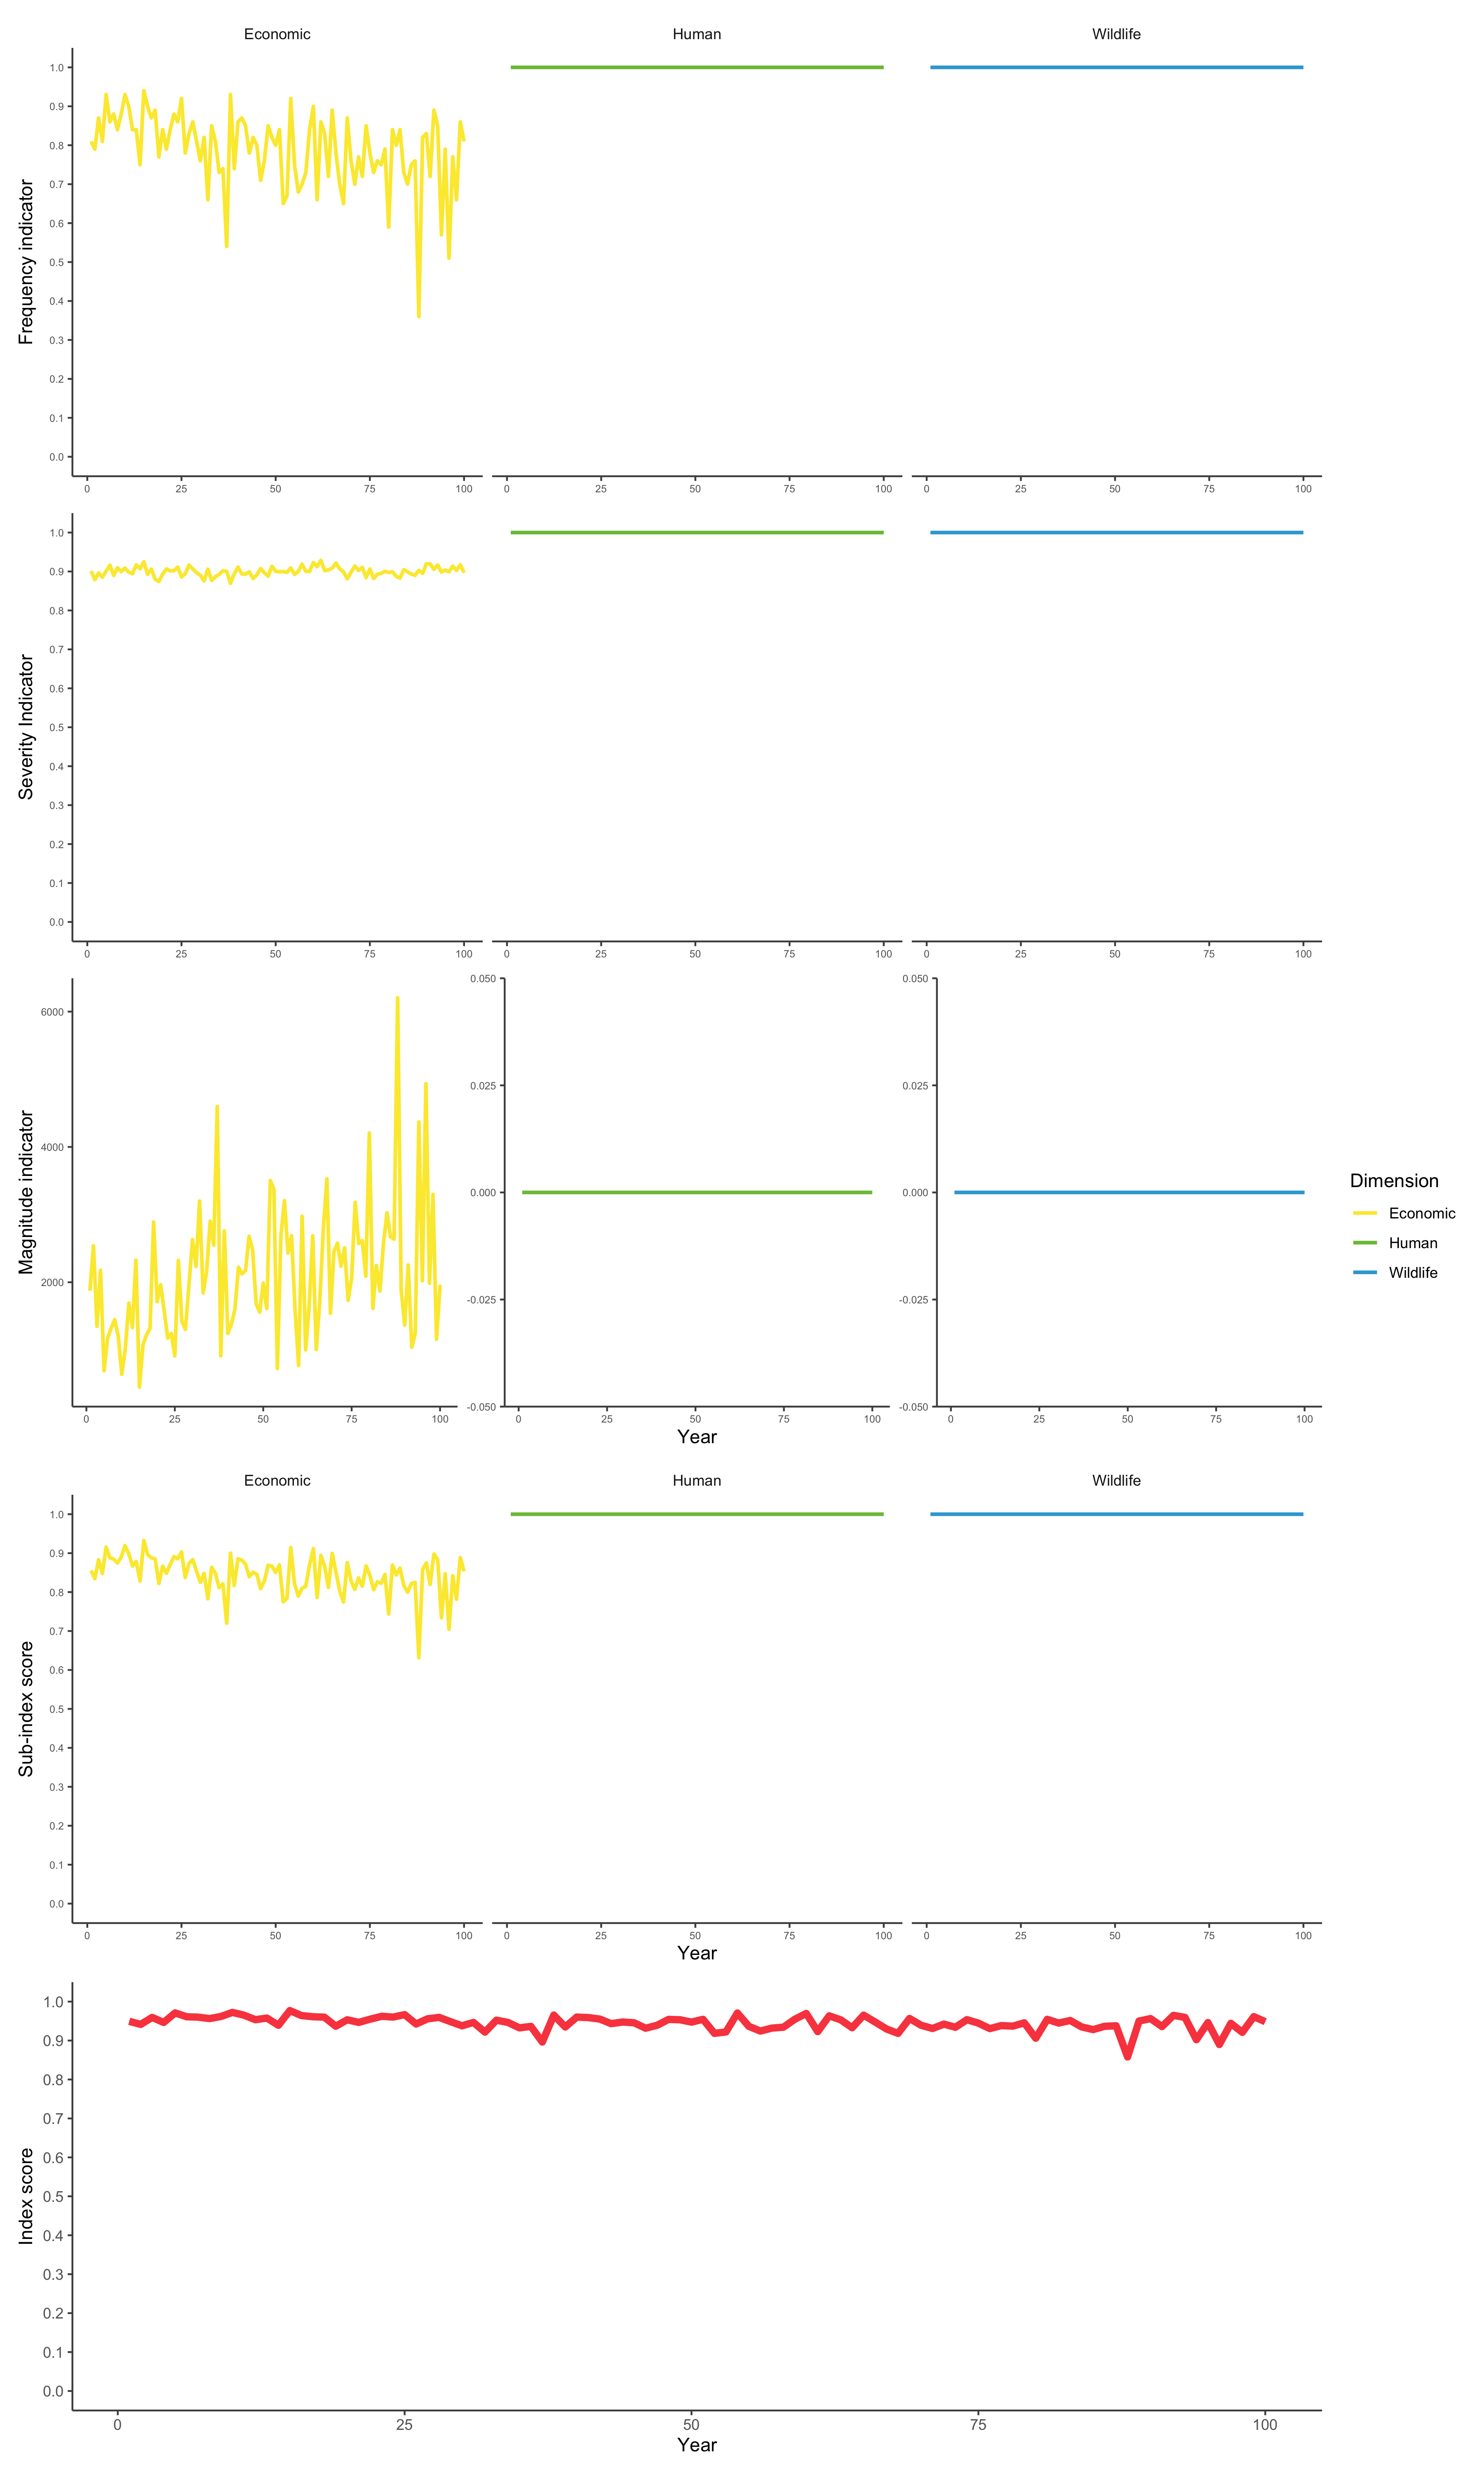
\includegraphics[width = 1\textwidth]{sp2_all.png}
    \caption{Indicators, sub-indices, and index of human-wildlife conflict for simulated Species 2}
    \label{fig:sp2}
\end{figure}

\subsubsection*{Species 3}
Species 3 shows movement across all indicators \ref{fig:sp3}, with declines in the human- and economic- dimension frequency and severity indicators, and increases in those magnitude indicators, while the wildlife-dimension indicators remain fairly stable, with only large movement on the severity indicator in a year where no widlife-victim incidents occurr.

\begin{figure}
    \centering
    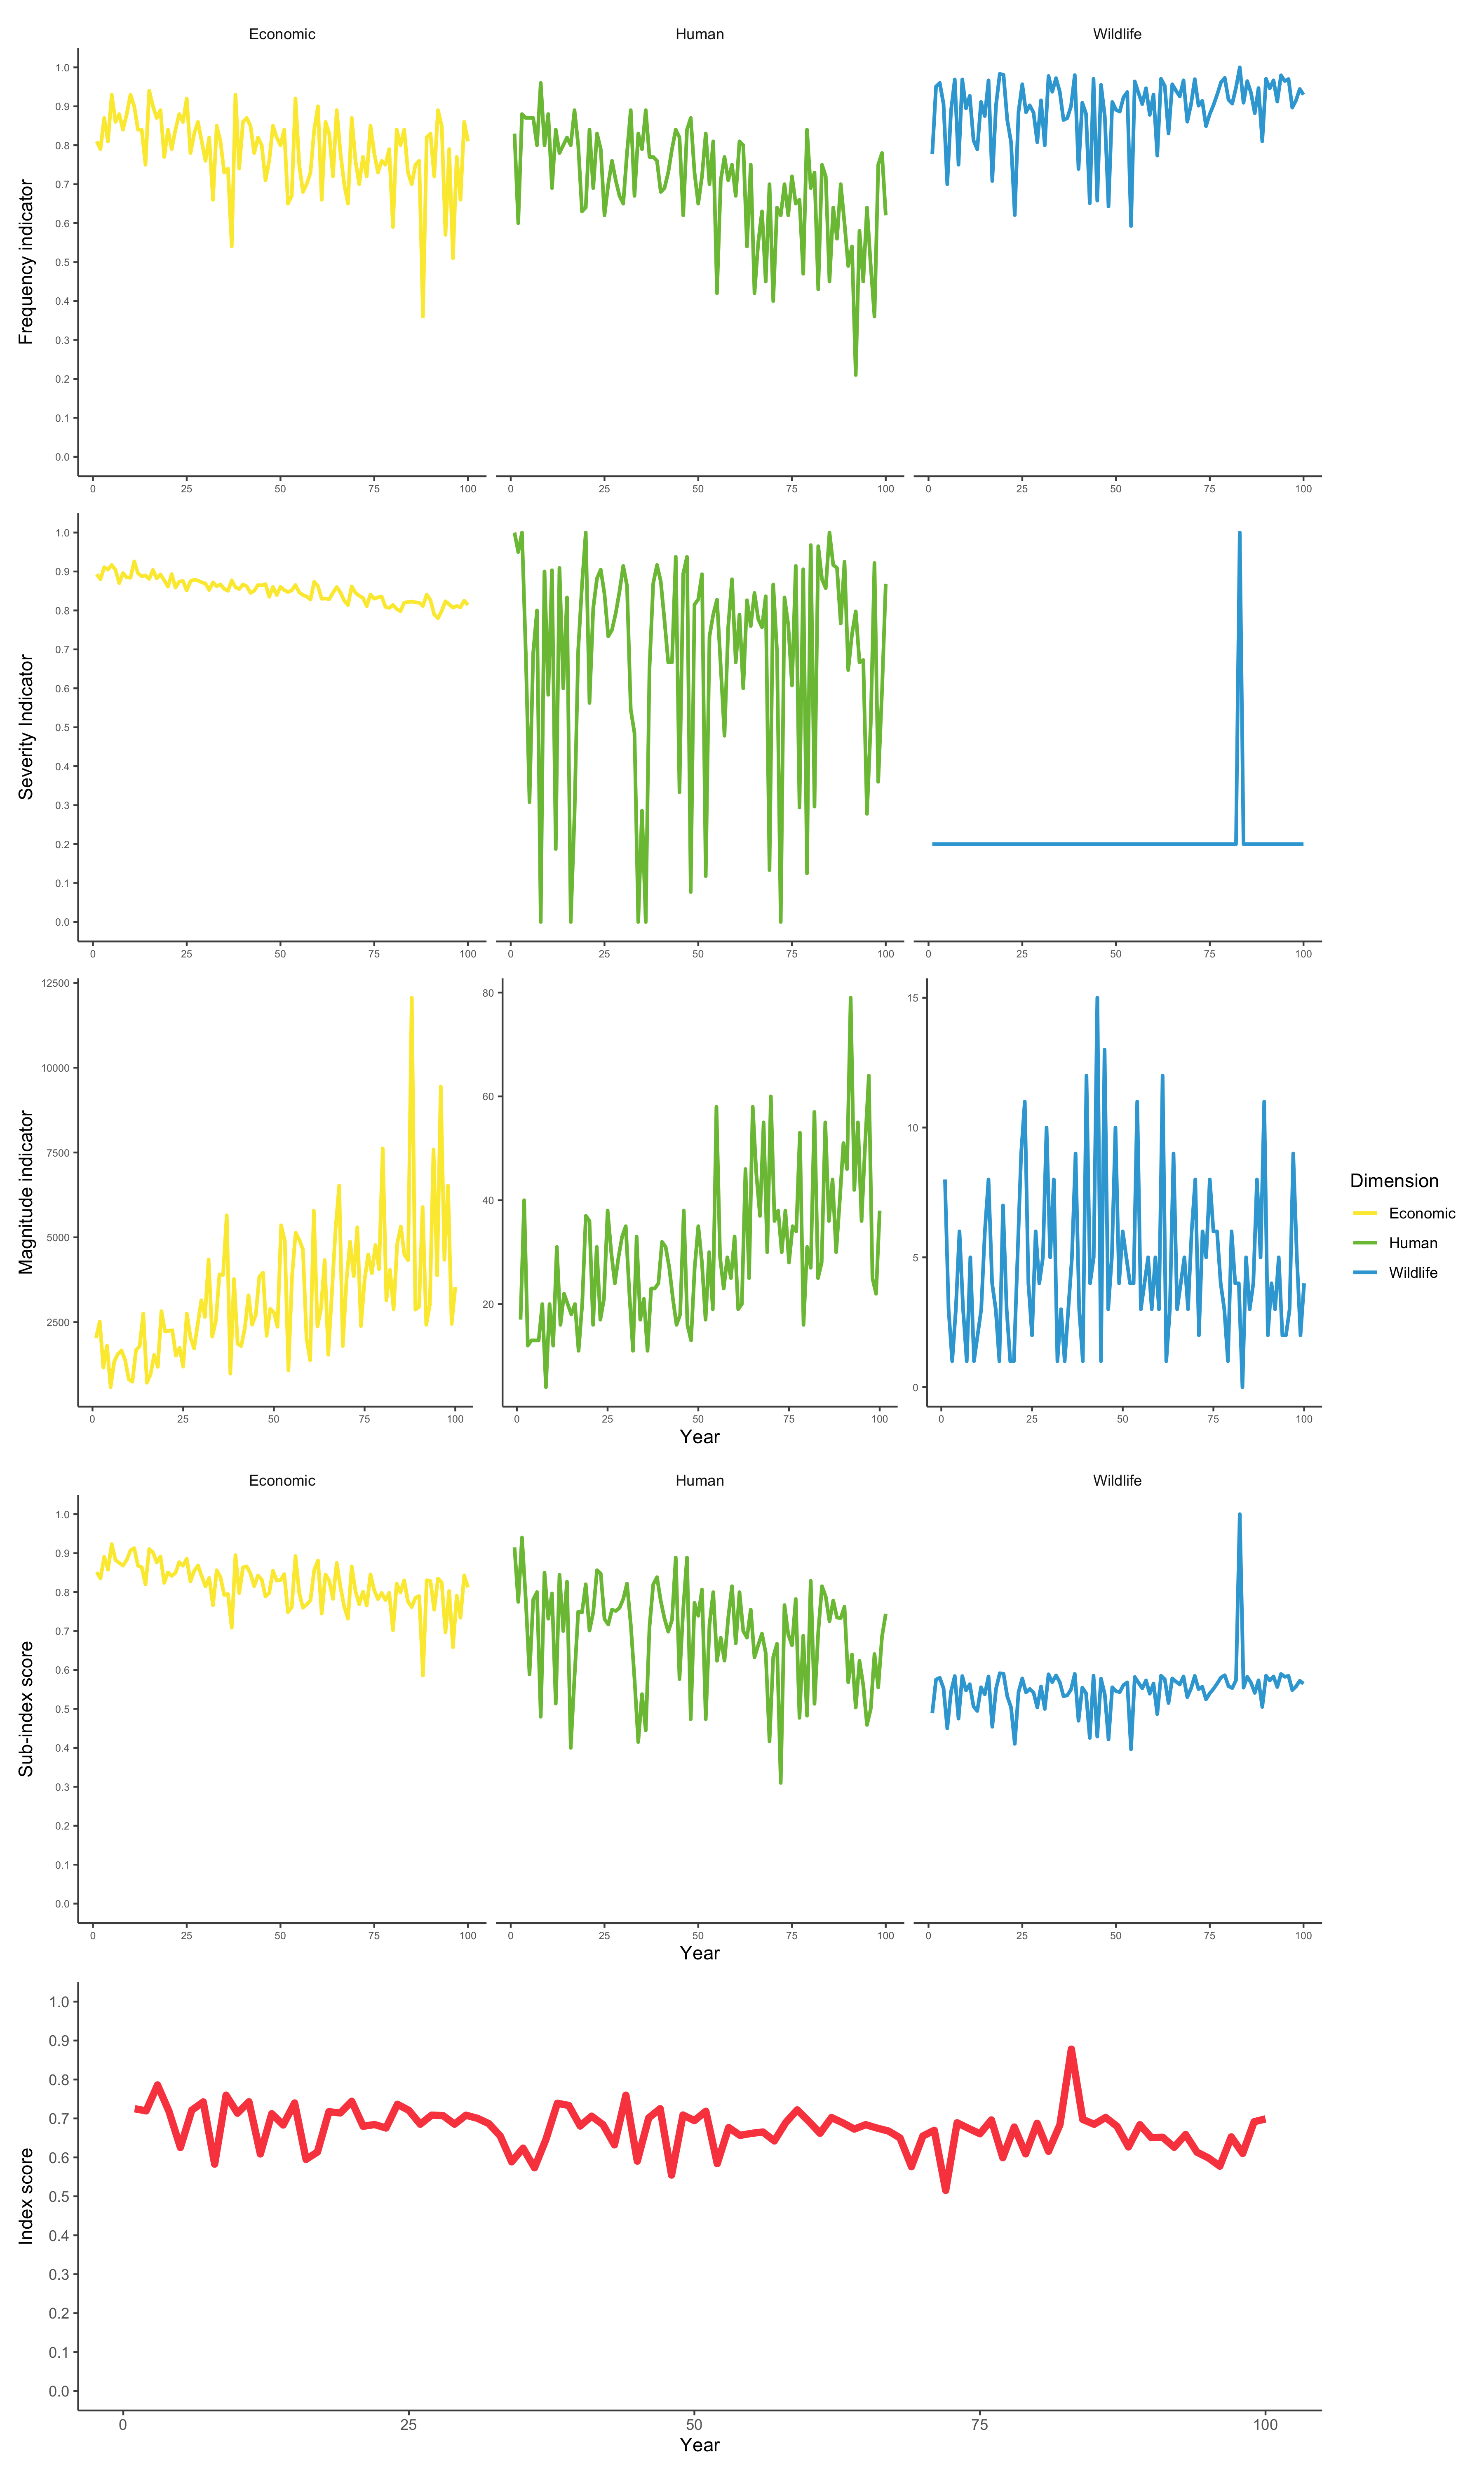
\includegraphics[width = 1\textwidth]{sp3_all.png}
    \caption{Indicators, sub-indices, and index of human-wildlife conflict for simulated Species 3}
    \label{fig:sp3}
\end{figure}

\subsubsection*{Landscape index}
The landscape index is generally stable with a slow decline \ref{fig:lsc} but drops rapidly to zero where the species 1 index equals zero, reflecting serious problems in the landscape in those years.

\begin{figure}
    \centering
    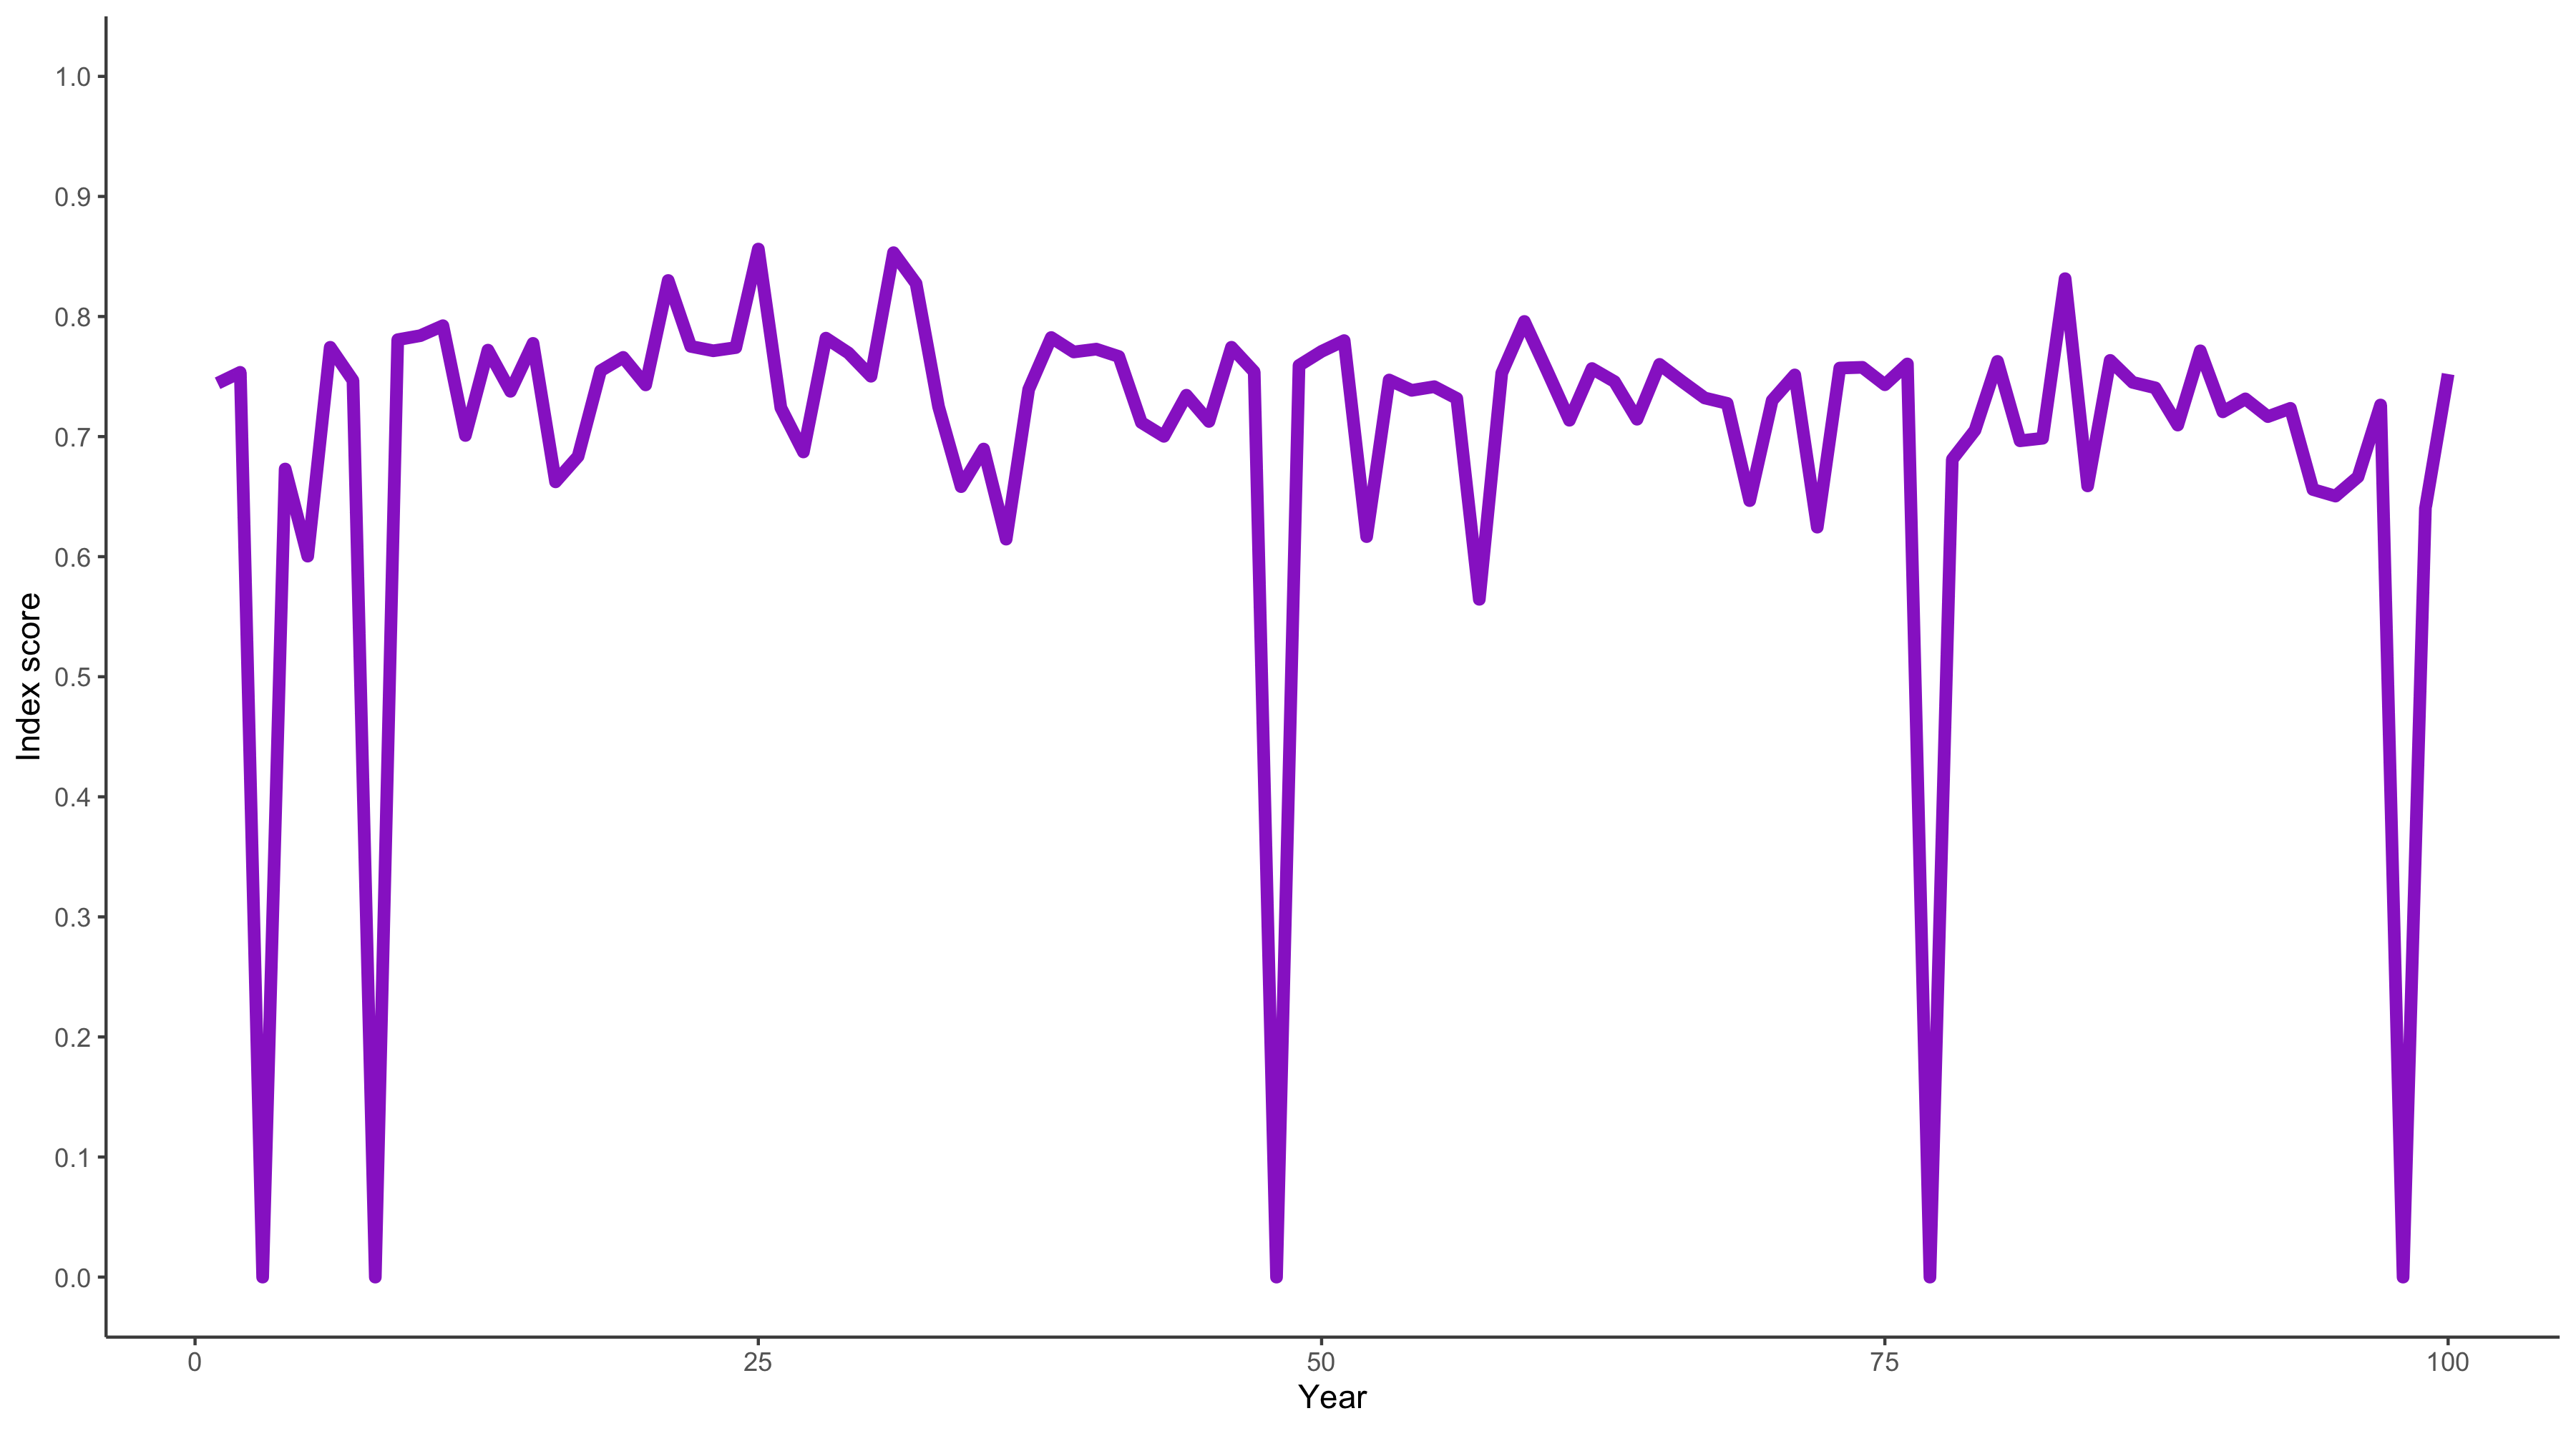
\includegraphics[width = 1\textwidth]{lsc_ix.png}
    \caption{Landscape index of human-wildlife conflict for simulated species 1, 2, and 3.}
    \label{fig:lsc}
\end{figure}

\subsection*{Human-Wildlife Conflict in Nepal}
For Nepal we calculated index suite values for Asian elephant \emph{Elephas maximus} \ref{fig:elephant}, tiger \emph{Panthera tigris} \ref{fig:tiger}, greater one-horned rhinoceros \emph{Rhinoceros unicornis} \ref{fig:rhino}, and wild pig \emph{Sus scrofa} \ref{fig:boar}. The latter two figures are found in the supplement. These combine to make an overall landscape index of human-wildlife conflict for Nepal for the years 2006--2016 \ref{fig:nepal}.

In general, the frequency indicators look flat for all dimensions in all years in Nepal --- in fact they are moving but very close to one, reflecting the relatively small number of recorde HWC indidents compared with the population of Nepal. The wildlife-dimension indicators are also flat and equal to one for frequency and severity, and zero for magnitude, as there are no records of wildlife-victim incidents (e.g. reprisal killings of wildlife) in this period e.g. \ref{fig:elephant}, \ref{fig:tiger}.

The index values for all species and the landscape are high, reflecting the relatively low levels of human-wildlife conflict in the country when compared with the overall populations of humans and wildlife \ref{fig:nepal} 

\begin{figure}
    \centering
    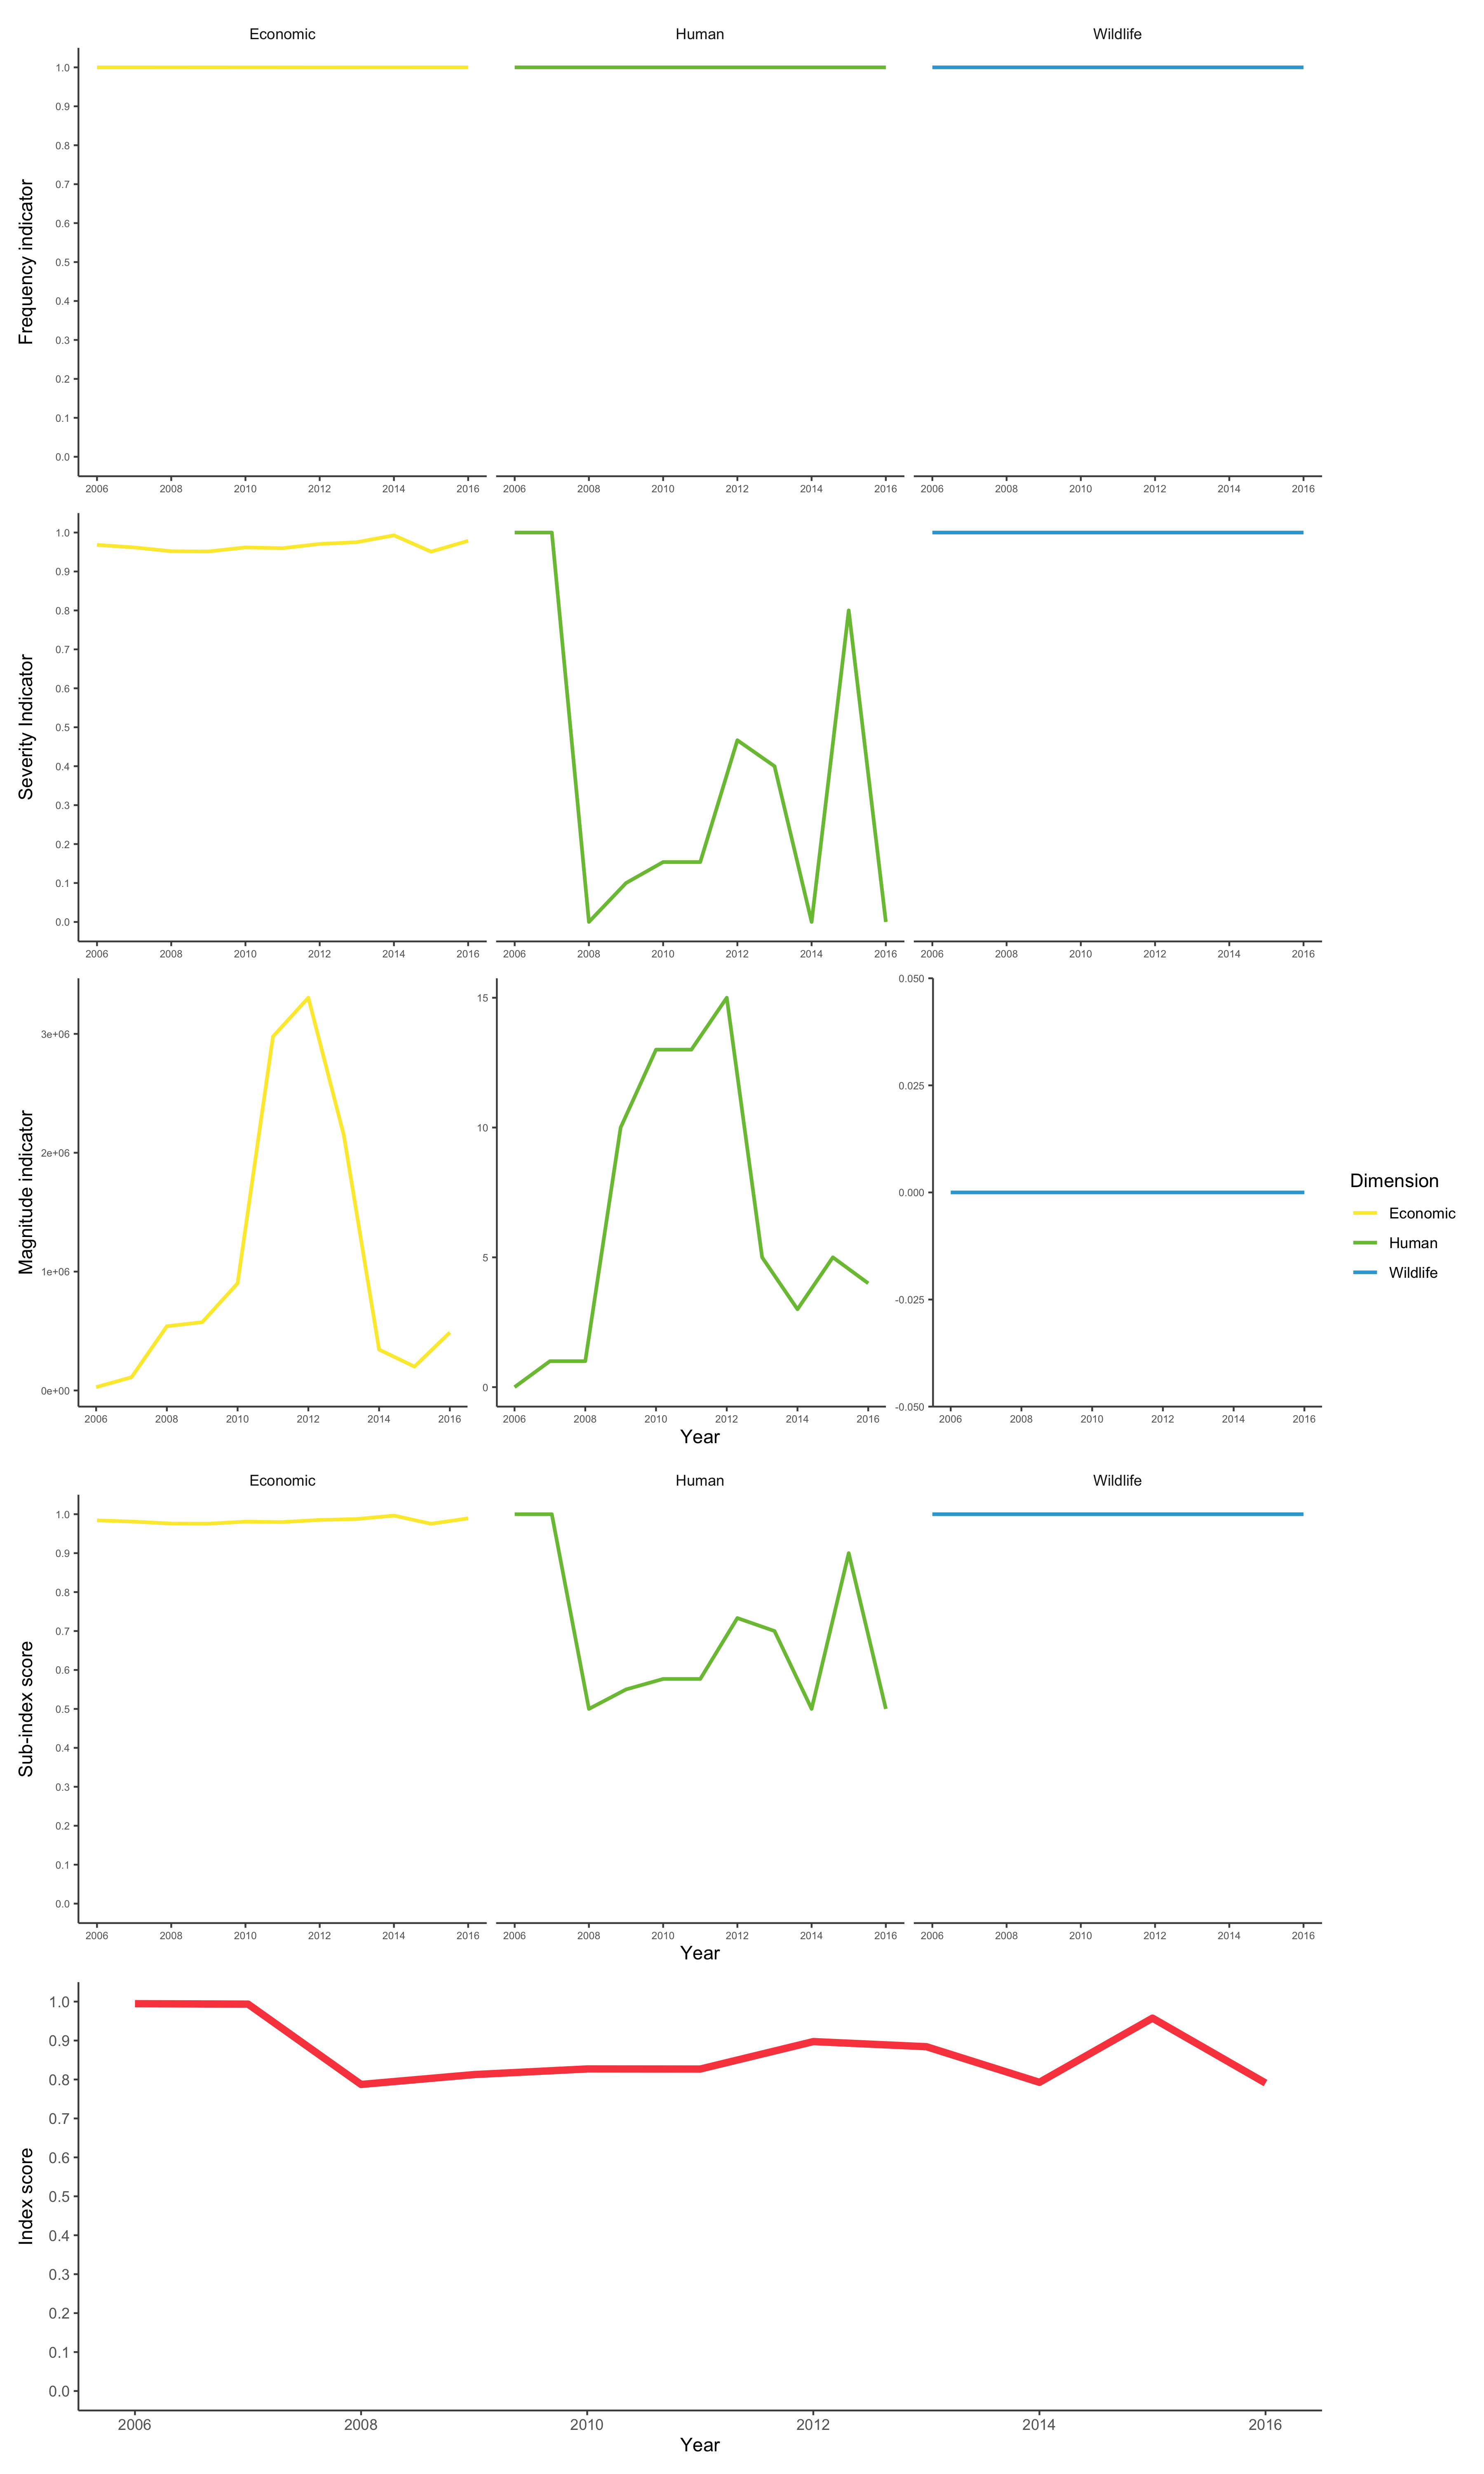
\includegraphics[width = 1\textwidth]{elephant_all.png}
    \caption{Indicator suite for Asian elephants in Nepal.}
    \label{fig:elephant}
\end{figure}

\begin{figure}
    \centering
    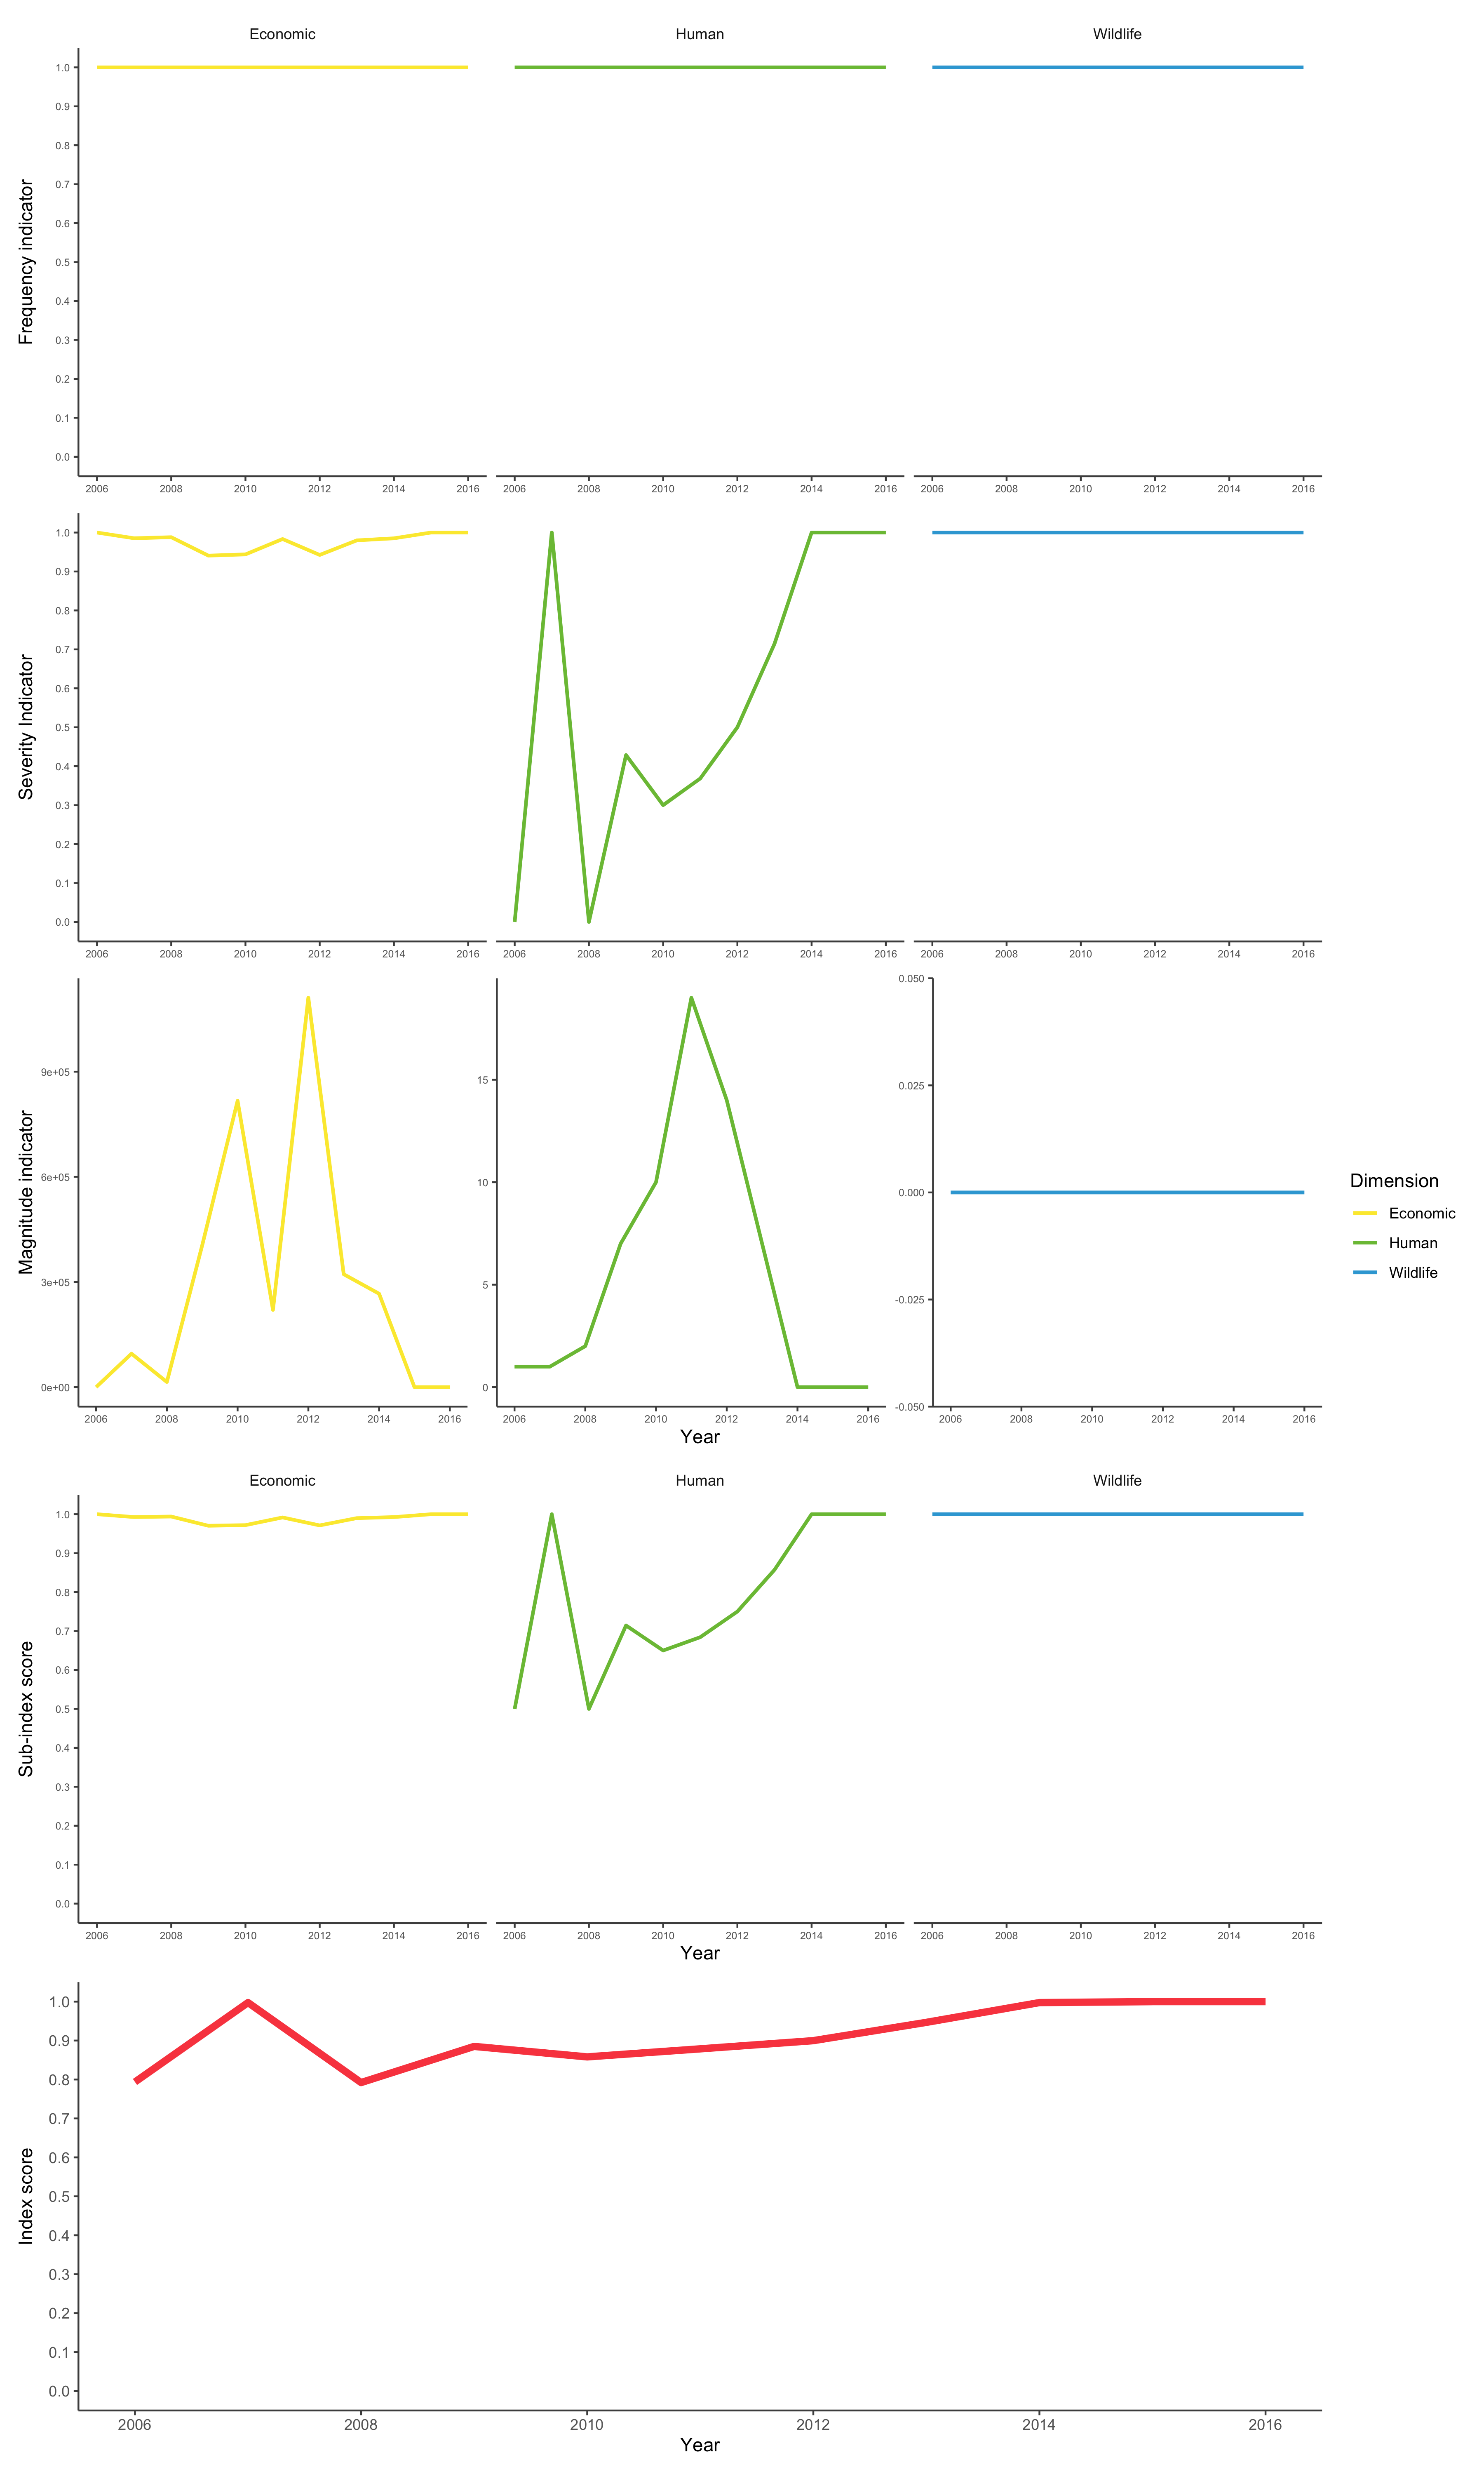
\includegraphics[width = 1\textwidth]{tiger_all.png}
    \caption{Indicator suite for tigers in Nepal.}
    \label{fig:tiger}
\end{figure}

\begin{figure}
    \centering
    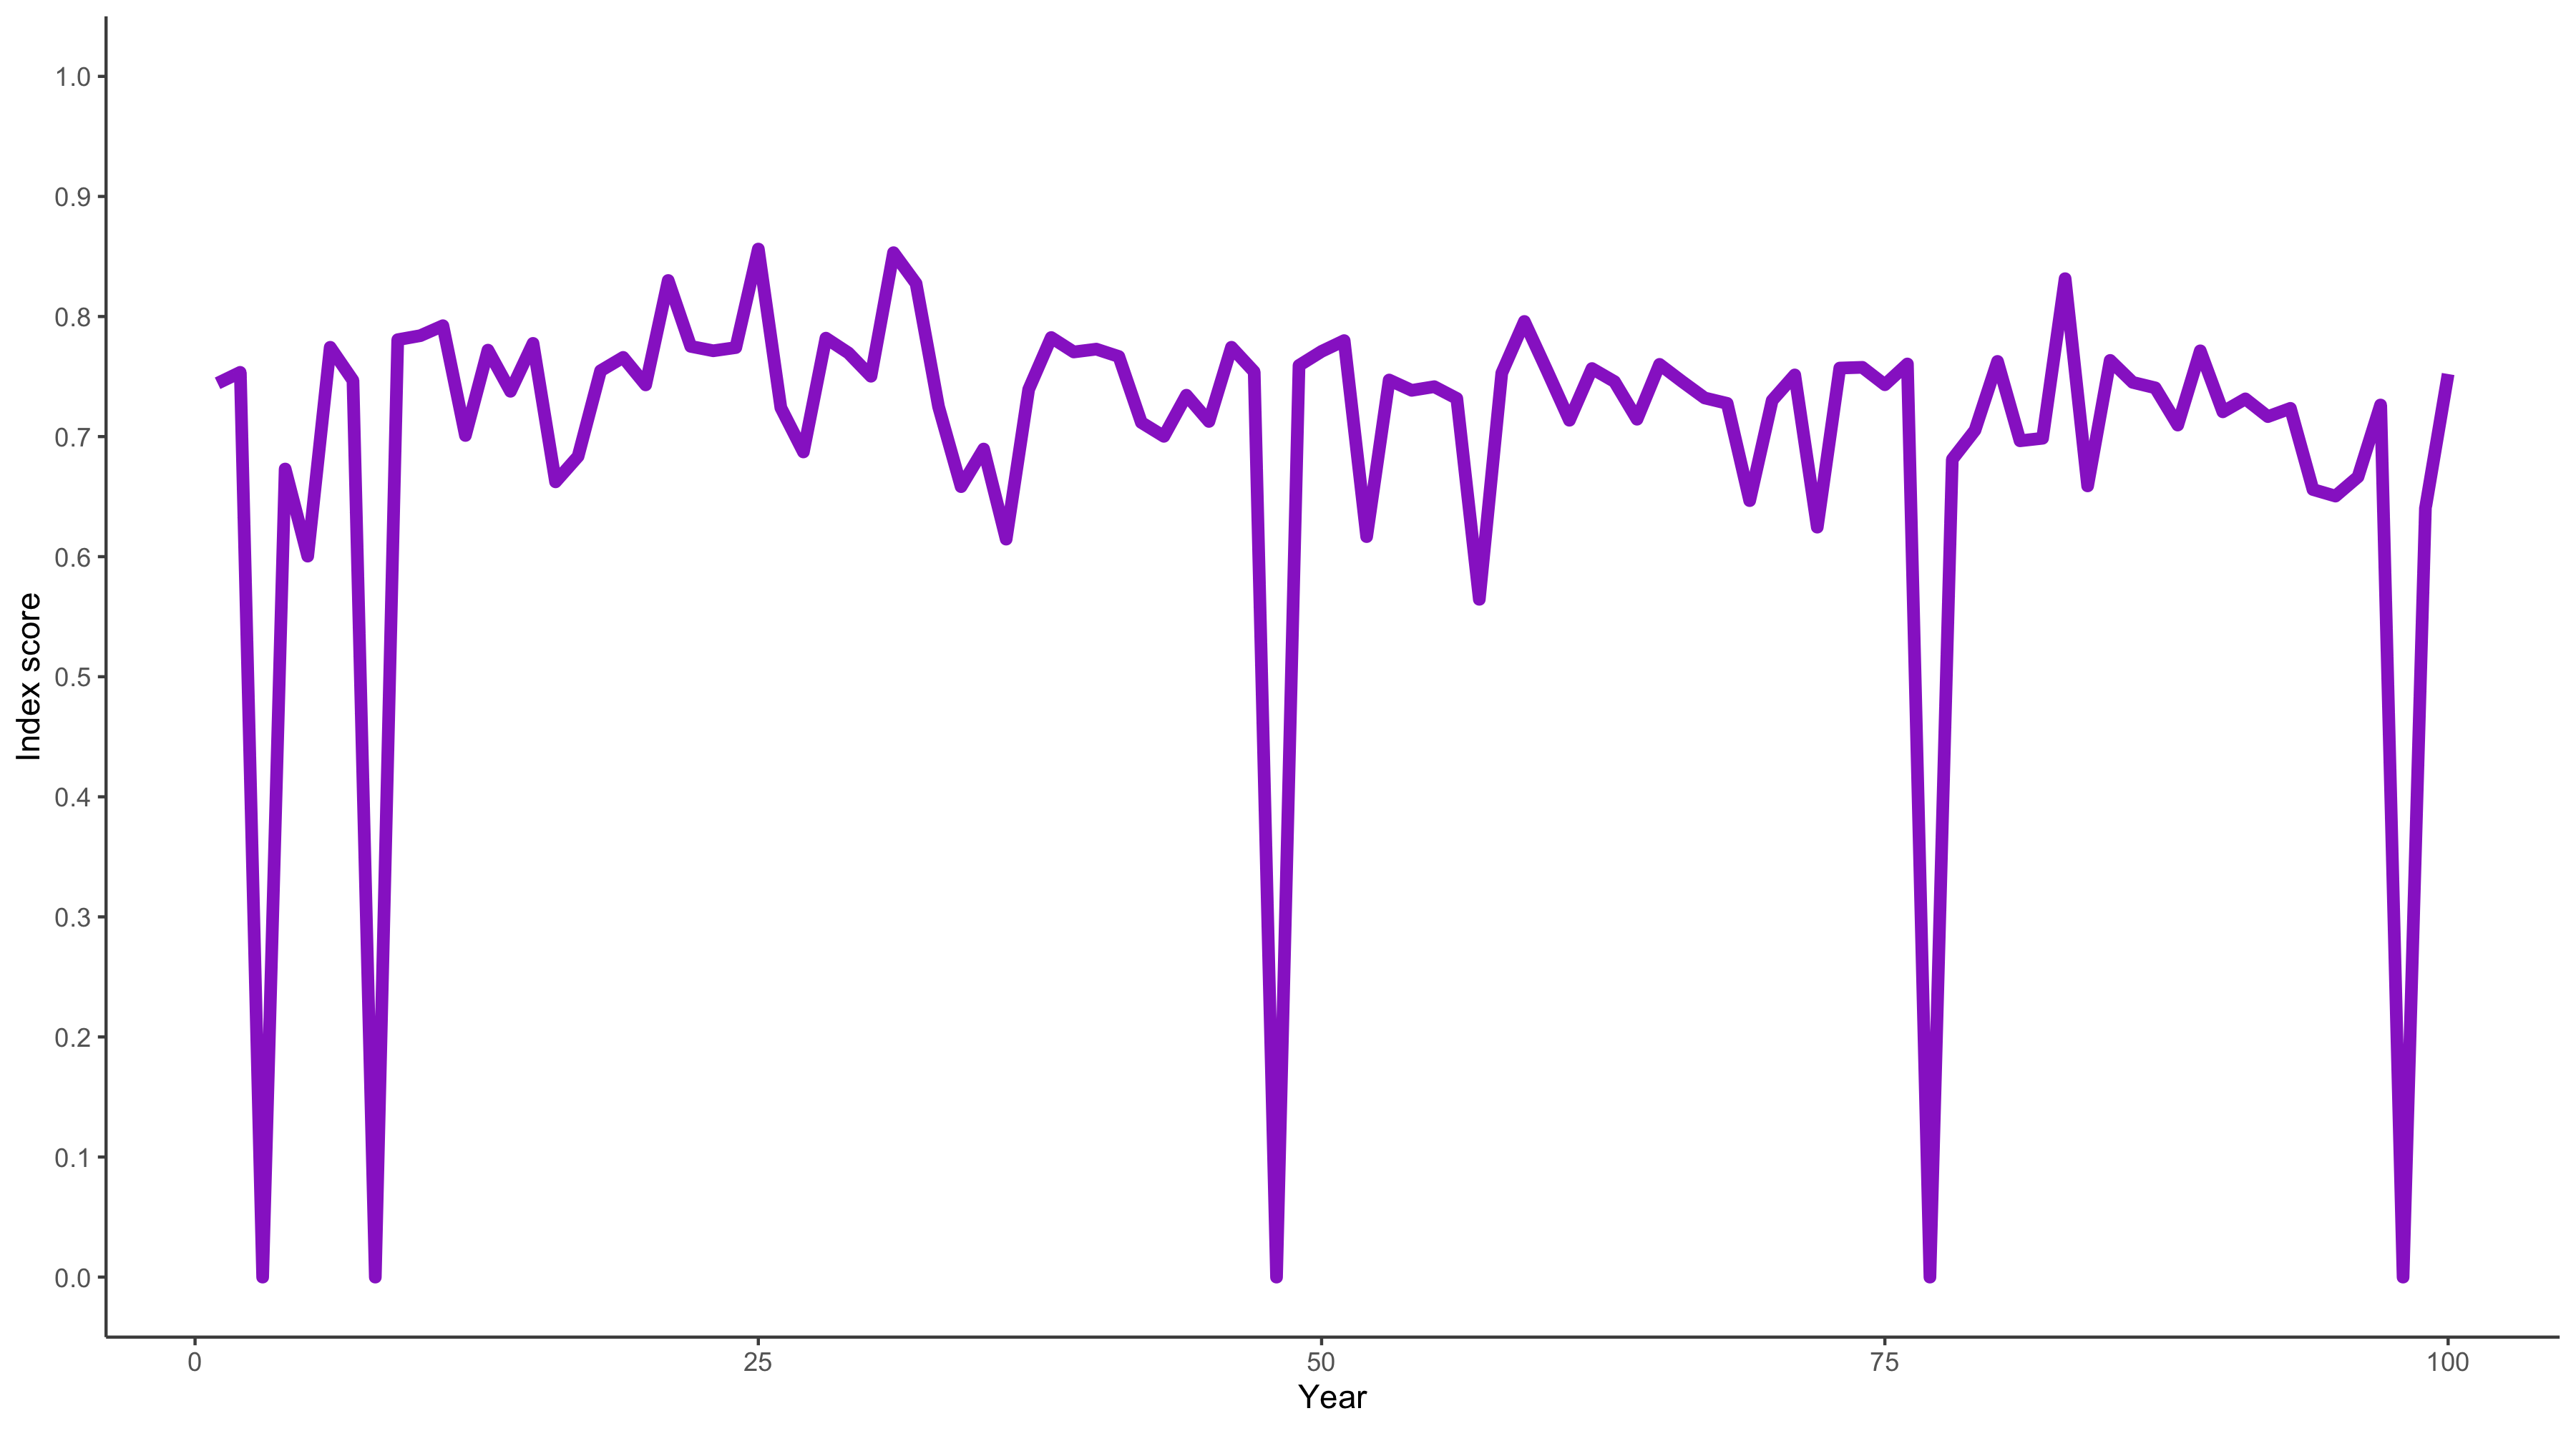
\includegraphics[width = 1\textwidth]{nepal_ix.png}
    \caption{Landscale index of human-wildlife conflict for Nepal, 2006--2016.}
    \label{fig:nepal}
\end{figure}

%\subsection*{Human-Elephant Conflict in Sabah, Malaysia}

%\bibliographystyle{unsrtnat}        
%\bibliography{refs}

%%%%%%%%%%%%%%%%%%%%%%%%%%%%
% APPENDIX
%%%%%%%%%%%%%%%%%%%%%%%%%%%%
\clearpage
\appendix
\renewcommand\thefigure{S\arabic{figure}}
\renewcommand\thetable{S\arabic{table}}
\renewcommand\theequation{S\arabic{equation}}
\setcounter{figure}{0}
\setcounter{table}{0}

\section*{Supplement: Index formulation and calculation}
\label{S1}
Index formulation
In this section we provide details of the calculation of the index. For each indicator, sub-index, and the index, we provide a description of the calculation, an equation, and a brief description of the item and reasoning for its construction. Symbols used in the equations are detailed below in Table \ref{tab:index_params}.


\begin{table}[ht!]
    \centering
    \caption{Key terms and definitions}
    \label{tab:definitions}
    \begin{tabular}{
    >{\raggedright\arraybackslash}p{3.5cm}
    p{10cm}
    }
         Wildlife-victim incident & A discrete event where wildlife are harmed as a result of HWC, e.g., killed or harmed as reprisals for damage to crops.\\
         Human-victim incident & A discrete event where humans are harmed by wildlife, ranging from minor incidents such as fear, to major incidents like mortalities.\\
         Economic incident & A discrete event resulting in economic losses such as damage to crops or infrastructure.\\
         Human-centric incident & Human-victim or economic incidents.\\
         HWC incident & Any type of human-victim, wildlife-victim or economic incident.\\
         
    \end{tabular}
\end{table}

\begin{table}[!ht]
    \centering
    \caption{Definitions of parameters used in used in equations in supplement \ref{S1} for HWC indicators and indices.}
    \label{tab:index_params}
    \begin{tabular}{p{1cm} p{13cm}}
         $\Psi$ & Landscape Human-wildlife Conflict Index \\
         $X$ ($X_\iota$) &	Species Human-wildlife Conflict Index (for species $\iota$) \\
         $\chi_h$ &	Human dimension sub-index \\
         $\chi_e$ &	Economic dimension sub-index \\
         $\chi_w$ &	Wildlife dimension sub-index \\
         $H_f$ &	one minus the probability of human-victim incidents \\
         $H_f^\ast$ &  Approximation of $H_f$ \\
         $H_s$ &	One minus the proportion of human-victim incidents that are human mortalities \\
         $H_m$ &	Number of human incidents \\
         $E_f$ &	One minus the probability of economic incidents \\
         $E_f^\ast$ &  Approximation of $E_f$ \\
         $E_s$ &	One minus the proportion of economic loss \\
         $E_m$ &	Net economic loss \\
         $W_f$ &	One minus the probability of wildlife-victim incidents (reprisal killings) given human-centric HWC incidents \\
         $W_s$ &	Are wildlife-victim incidents occurring given IUCN Red List status  \\
         $W_m$ &	Number of wildlife-victim incidents \\
         $j$ & Number of households in the landscape \\
         $m$ &	Number of human mortalities in landscape \\
         $u$ &	Number of households experiencing any human-victim incidents in landscape (including human mortalities). \\
         $v$ &	Number of human-victim incidents in landscape (including human mortalities) \\
         $a$ &	Number of households experiencing economic incidents in the landscape \\
         $b$ &	Number of economic incidents in the landscape \\
         $l_i$ &	Net economic loss of entity (household) i \\
         $w_i$ &	Net wealth of entity (household) i \\
         $\overline{w}$ & Mean household wealth in landscape \\
         $r$ &	Number of wildlife-victim incidents (e.g. reprisal killings of wildlife) in the landscape \\
         $s$ & IUCN Red List status of target species \\
         $\kappa$ & Number of target species in the landscape
    \end{tabular}
\end{table}


\subsection*{Human dimension}
\subsubsection*{Human dimension --- frequency indicator:}
This indicator, $H_f$, is defined the probability of a household experiencing one or more human-victim incidents. $H_f$, is calculated as the number of households experiencing human-victim incidents in the landscape, $u$, divided by the number of households in the landscape, $j$:
\begin{equation*}
    H_f = u/j
\end{equation*}

where $H_f \in [0,1]$ and zero is the desired state, i.e. no human-victim incidents are occurring.\\

For practical purposes, it may often not be possible to determine whether the same households experience repeated incidents in a given time-frame, or if records relate to different households. To simplify, if we assume that the total number of human-victim incidents $v$ approximates the number of households experiencing human-victim incidents, $v \simeq u$ (i.e., only one incident per household), then we may approximate $H_f^\ast \simeq H_f$ where:

\begin{equation*}
    H_f^\ast = \begin{cases}
        1       & v > j \\
        v/j & v \le j \\
    \end{cases}
\end{equation*}

and $H_f^\ast \in [0,1]$.\\

It is likely that for most purposes it will only be possible or calculate $H_f^\ast$.


\subsubsection*{Human dimension --- severity indicator:}
This indicator, $H_s$ is defined as the proportion of human-victim incidents that result in human mortality. $H_s$ is calculated as the number of human mortalities, $m$, divided by the number of human-victim incidents, $v$:

\begin{equation*}
    H_s = \begin{cases}
        1 & m > v \\
        m/v & v \ge m > 0 \\
        0       & m = 0 \\
    \end{cases}
\end{equation*}



where $H_s \in [0,1]$ and zero is the desired state, i.e. no human-victim incidents are occurring. 

Constraints on the ranges of $v$ and $m$ are necessary for two reasons: firstly, because if no human-victim incidents occur the indicator should be in it's desired state, but a denominator of zero is undefined, and secondly,  because incidents may involve multiple victims, but the numerator $m$ is a count of total mortalities, the indicator could otherwise become greater than one.

This indicator is intended as a coarse measure of the relative severity of incidents, counting the proportion of human incidents that result in mortality. Hs will range from one, where no incidents are mortalities, to zero, when all incidents result in the loss of a human life. This measure will be unable to differentiate among incidents less severe than mortalities, e.g., comparing the loss of a limb to a shark to being intimidated by a swooping bird. This coarseness is intentional because it makes the indicator easy to understand and calculate, and it avoids the need to make difficult, equivocal, or value-laden judgements about the relative severity of a range of incidents. In some cases however this could result in indicator values that appear to indicate a low level of severity, however may mask other differences among landscapes, e.g. frequent physical attacks resulting in human injuries on one landscape but not in another would not be differentiated by this measure. It is important that this context is maintained elsewhere, such as through other appropriate context indicators.

\subsubsection*{Human dimension --- magnitude indicator:}
This indicator $H_m$ is simply defined as the number of human-victim incidents in the landscape:

\begin{equation*}
    H_m = v
\end{equation*}

where $H_m \in [0,\infty)$, and the desired state is zero.
This measure is also a coarse measure that is quick to calculate and easy to understand. The magnitude of the problem will be relative to the scale of the landscape, so it may not be reasonable to directly compare this indicator across landscapes of different sizes, however it will be useful for grasping the overall scale of the problem in a given landscape.

\subsubsection*{Human dimension --- sub-index:}

This sub-index $\chi_h$ is calculated as the arithmetic mean of  the human-dimension frequency and severity indicators:

\begin{equation*}
    \chi_h = \frac{H_f + H_s}{2}
\end{equation*}

where $\chi_h \in [0,1]$ and zero is the desired state. This sub-index equally weights and aggregates the frequency and severity measures.

\subsection*{Economic dimension}

\subsubsection*{Economic dimension --- frequency indicator:}
This indicator, $E_f$, is defined as  the probability of an household experiencing one or more economic incidents. $E_f$, is calculated as the number of households experiencing economic incidents in the landscape, $a$, divided by the number of households in the landscape, $j$:

\begin{align*}
    E_f = a/j
\end{align*}

where $E_f \in [0,1]$ and zero is the desired state, i.e. no economic incidents are occurring.\\

As with $H_f$, it may often not be possible to determine whether the same households experience repeated incidents in a given time-frame, or if records relate to different households. Economic incidents may also effect entities other than households, for example businesses. However if we assume that the total number of economic incidents approximates the number of households experiencing economic incidents, $b \simeq a$, then we may approximate $E_f^\ast \simeq E_f$ where:

\begin{equation*}
    E_f^\ast = \begin{cases}
        1        & b > j \\
        b/j  & b \le j \\
    \end{cases}
\end{equation*}

and $E_f^\ast \in [0,1]$.\\

It is likely that for most purposes it will only be possible or calculate $E_f^\ast$.

\subsubsection*{Economic dimension --- severity indicator:}
This indicator $E_s$ is defined as the landscape arithmetic mean over each entity in the in the landscape which experienced economic loss due to HWC, $a$, of the net entity (household) economic loss, $l_i$, divided by entity (household) economic wealth, $w_i$:

\begin{align*}
    E_s = \begin{cases}
        \sum_{i=1}^{j}(\frac{l_i}{w_i})/a & a > 0 \\
        0                                     & a = 0
    \end{cases}
\end{align*}

where $E_s \in [0,1]$, and zero is the desirable state. \\ 

An entity in this case is considered either a household or business. The purpose of this delineation to entity level wealth $w_i$ is intended to make the index sensitive to the wealth of the those effected by HWC. If poorer households are disproportionately effected by HWC, the use of some a landscape average of wealth, $\overline{w}$, will mask the severity of the incidents relative to the household effected. Conversely if large companies tend to be the victims, all things being equal then such landscape averages will overstate the problem. \\

However as with other indicators, it may not be practical to know either the entity wealth, $w_i$, or the exact number of entities that are victims of economic incidents. Again if we again assume  that the total number of economic incidents approximates the number of entities experiencing economic incidents, $b \simeq a$, and use a landscape-level average household wealth $\overline{w}$, then we may approximate $E_s^\ast \simeq E_s$ where:

\begin{equation*}
    E_s^\ast = \begin{cases}
    1                   & b > 0,\; \sum_{i=1}^{j}(\frac{l_i}{\overline{w}})/b > 1\\
    \sum_{i=1}^{j}(\frac{l_i}{\overline{w}})/b & b > 0,\; \sum_{i=1}^{j}(\frac{l_i}{\overline{w}})/b \le 1 \\
    0                   & b = 0 \\
    \end{cases}
\end{equation*}

and $E_s \in [0,1]$.\\

\subsubsection*{Economic dimension --- magnitude indicator:}

This indicator $E_m$ is defined as the net economic loss in the landscape, and calculated as the sum of all household economic loss in the landscape:

\begin{equation*}
    E_m = \sum_{i=1}^{j}l_i
\end{equation*}

The indicator can be defined in any arbitrary unit or local currency, however the same unit must be used to allow comparisons among landscapes.

\subsubsection*{Economic dimension --- sub-index:}

This sub-index $\chi_e$ is calculated as the arithmetic mean of  the economic-dimension frequency and severity indicators:
\begin{equation*}
    \chi_e = \frac{E_f + E_s}{2}
\end{equation*}

where $\chi_e \in [0,1]$ and one is the desired state. This sub-index equally weights and aggregates the frequency and severity measures.

\subsection*{Wildlife}

\subsubsection*{Wildlife dimension --- frequency indicator:}

This indicator $W_f$ is considered as one minus the probability of wildlife-victim incidents (generally reprisal killing or otherwise harming of perceived perpetrator species) given HWC incidents. It is calculated as one minus the number of wildlife-victim incidents divided by the number of human-centric HWC incidents (human-victim incidents and economic incidents):

\begin{equation*}
    W_f = \begin{cases}
    0                   &  v +b > 0,\; r > v +b \\
    1 - \frac{r}{v + b} & v + b > 0,\; r \le v + b \\
    1                   & v + b = 0 \\
    \end{cases}
\end{equation*}

where $W_f \in [0,1]$ and one is the desired state. Reasons for constraining the values of $W_f$ based on $r$, $v$, $b$ are as per those given for constraining $H_s$.

\subsubsection*{Wildlife dimension --- severity indicator:}
This indicator $W_s$ is dependant on whether wildlife-victim incident are occurring, and the IUCN Red List status of the species, subspecies, or population of interest. The specific values of $W_s$ are prescribed:

\begin{equation*}
    W_s = \begin{cases}
    0   & r > 0, \; s = CR \\
    0.2 & r > 0, \; s = EN \\
    0.4 & r > 0, \; s = VU \\
    0.6 & r > 0, \; s = NT \\
    0.8 & r > 0, \; s \in (LC, NE, DD) \\
    1   & r = 0
    \end{cases}
\end{equation*}

where $W_s \in [0,1]$ and one is the desired state.

The scaling of risk between Red List status levels is not linear as implied by this 

\subsubsection*{Wildlife dimension --- magnitude indicator:}
This indicator $W_m$ is simply defined as the number of wildlife-victim incidents in the landscape, which will largely be retaliatory killings of the target species:

\begin{equation*}
    W_m = r
\end{equation*}

where $W_m \in [0,\infty)$, and the desired state is zero.

Like $H_m$, this indicator is a coarse measure that is quick to calculate and easy to understand. The magnitude of the problem will be relative to the scale of the landscape, so it may not be reasonable to directly compare this indicator across landscapes of different sizes, however it will be useful for grasping the overall scale of the problem in a given landscape.

\subsubsection*{Wildlife dimension --- sub-index:}

This sub-index $\chi_w$ is calculated as the arithmetic mean of  the wildlife-dimension frequency and severity indicators:
\begin{equation*}
    \chi_w = \frac{W_f + W_s}{2}
\end{equation*}

where $\chi_w \in [0,1]$ and one is the desired state. This sub-index equally weights and aggregates the frequency and severity measures.

\subsection*{Context dimension --- indicators:}
The context dimension is an opportunity to include a range of indicators relevant to the HWC context of a particular landscape that help to tell the story of HWC in that landscape. Example indicators could include proportion of forest or other habitat cover in a landscape, the population sizes of the target species, measures of urbanization, engagement or policy metrics, or any other measures that managers consider relevant. These are not used in the calculation of any sub-index or index and so the index and sub-indices will still be comparable among landscapes even if different key context indicators are used among landscapes or species.

\subsection*{Species Human-wildlife Conflict Index}
This index $X$ is defined as the geometric mean of the three sub-indices, $\chi_h$, $\ch_e$, and $\chi_w$:

\begin{equation*}
    X = \sqrt[3]{\chi_h \times \chi_e \times \chi_w}
\end{equation*}

where $X \in [0,1]$ and one is the desired state, with no HWC of any sort occurring in the landscape.\\

The aim of this index is to give a simple overview of the state of HWC across a complex range of different elements, which we term dimensions, and axes of impact within them. The index is one mechanism to do this. Like all composite indices however, it masks much nuance within the data set, which is why we propose and strongly advocate for its use along with the suite of indicators to allow managers to better understand specific landscapes.
Dimension sub-indices are equally weighted, improvements in one dimension will not compensate for deterioration of equal magnitude in other sub-indices because of the use of geometric aggregation. Therefore a high index scores must be the result of high scores in all sub-indices.

\subsection*{Landscape Human-wildlife Conflict Index}
This index $\Psi$ enables a landscape composition of target species indices into a single multi-species index. $\Psi$ is calculated as the geometric mean of the Species Human-wildlife Conflict Indices $X_\iota$c for each of the $\kappa$ target species in the landscape, where:

\begin{equation*}
    \Psi = \sqrt[\kappa]{\prod_{\iota=1}^{\kappa} X_\iota }
\end{equation*}

where $\Psi \in [0,1]$ and one is the desired state, with no HWC occurring for any species the landscape.\\


\section*{Supplement: Additional figures}
\begin{figure}[!ht]
    \centering
    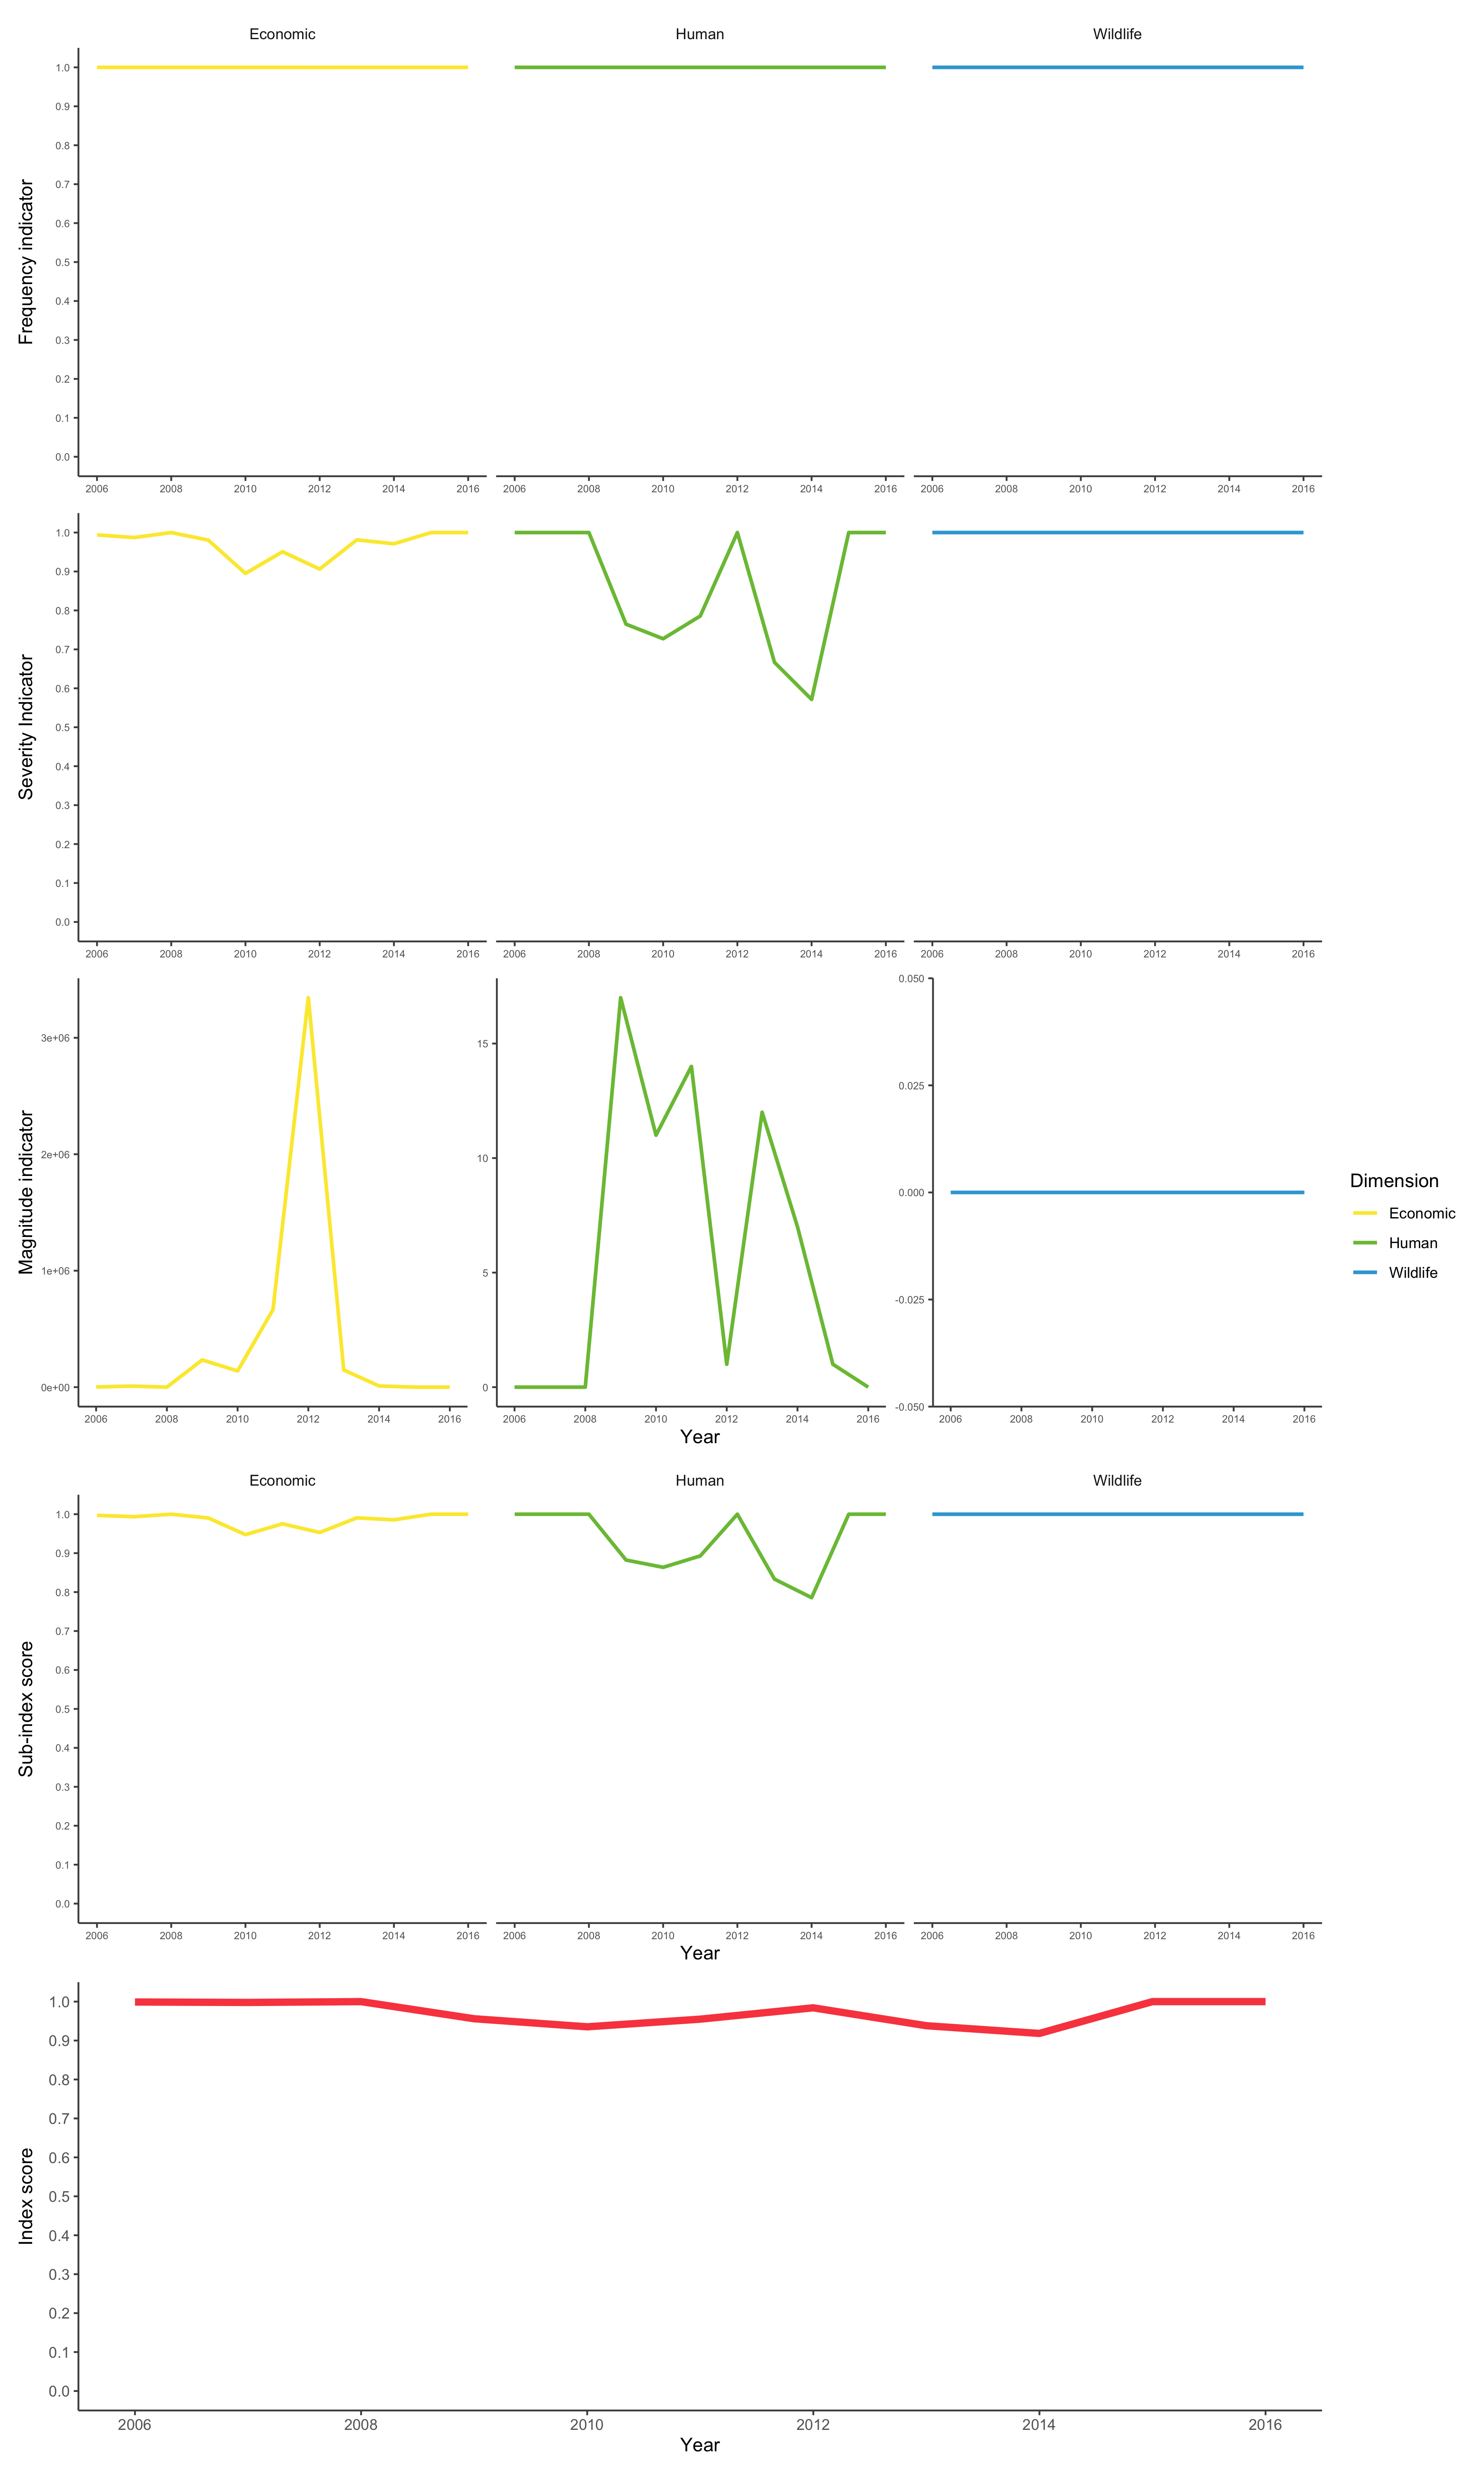
\includegraphics[width = 1\textwidth]{rhino_all.png}
    \caption{Indicator suite for Greater one-horned rhinoceros in Nepal.}
    \label{fig:rhino}
\end{figure}

\begin{figure}[!ht]
    \centering
    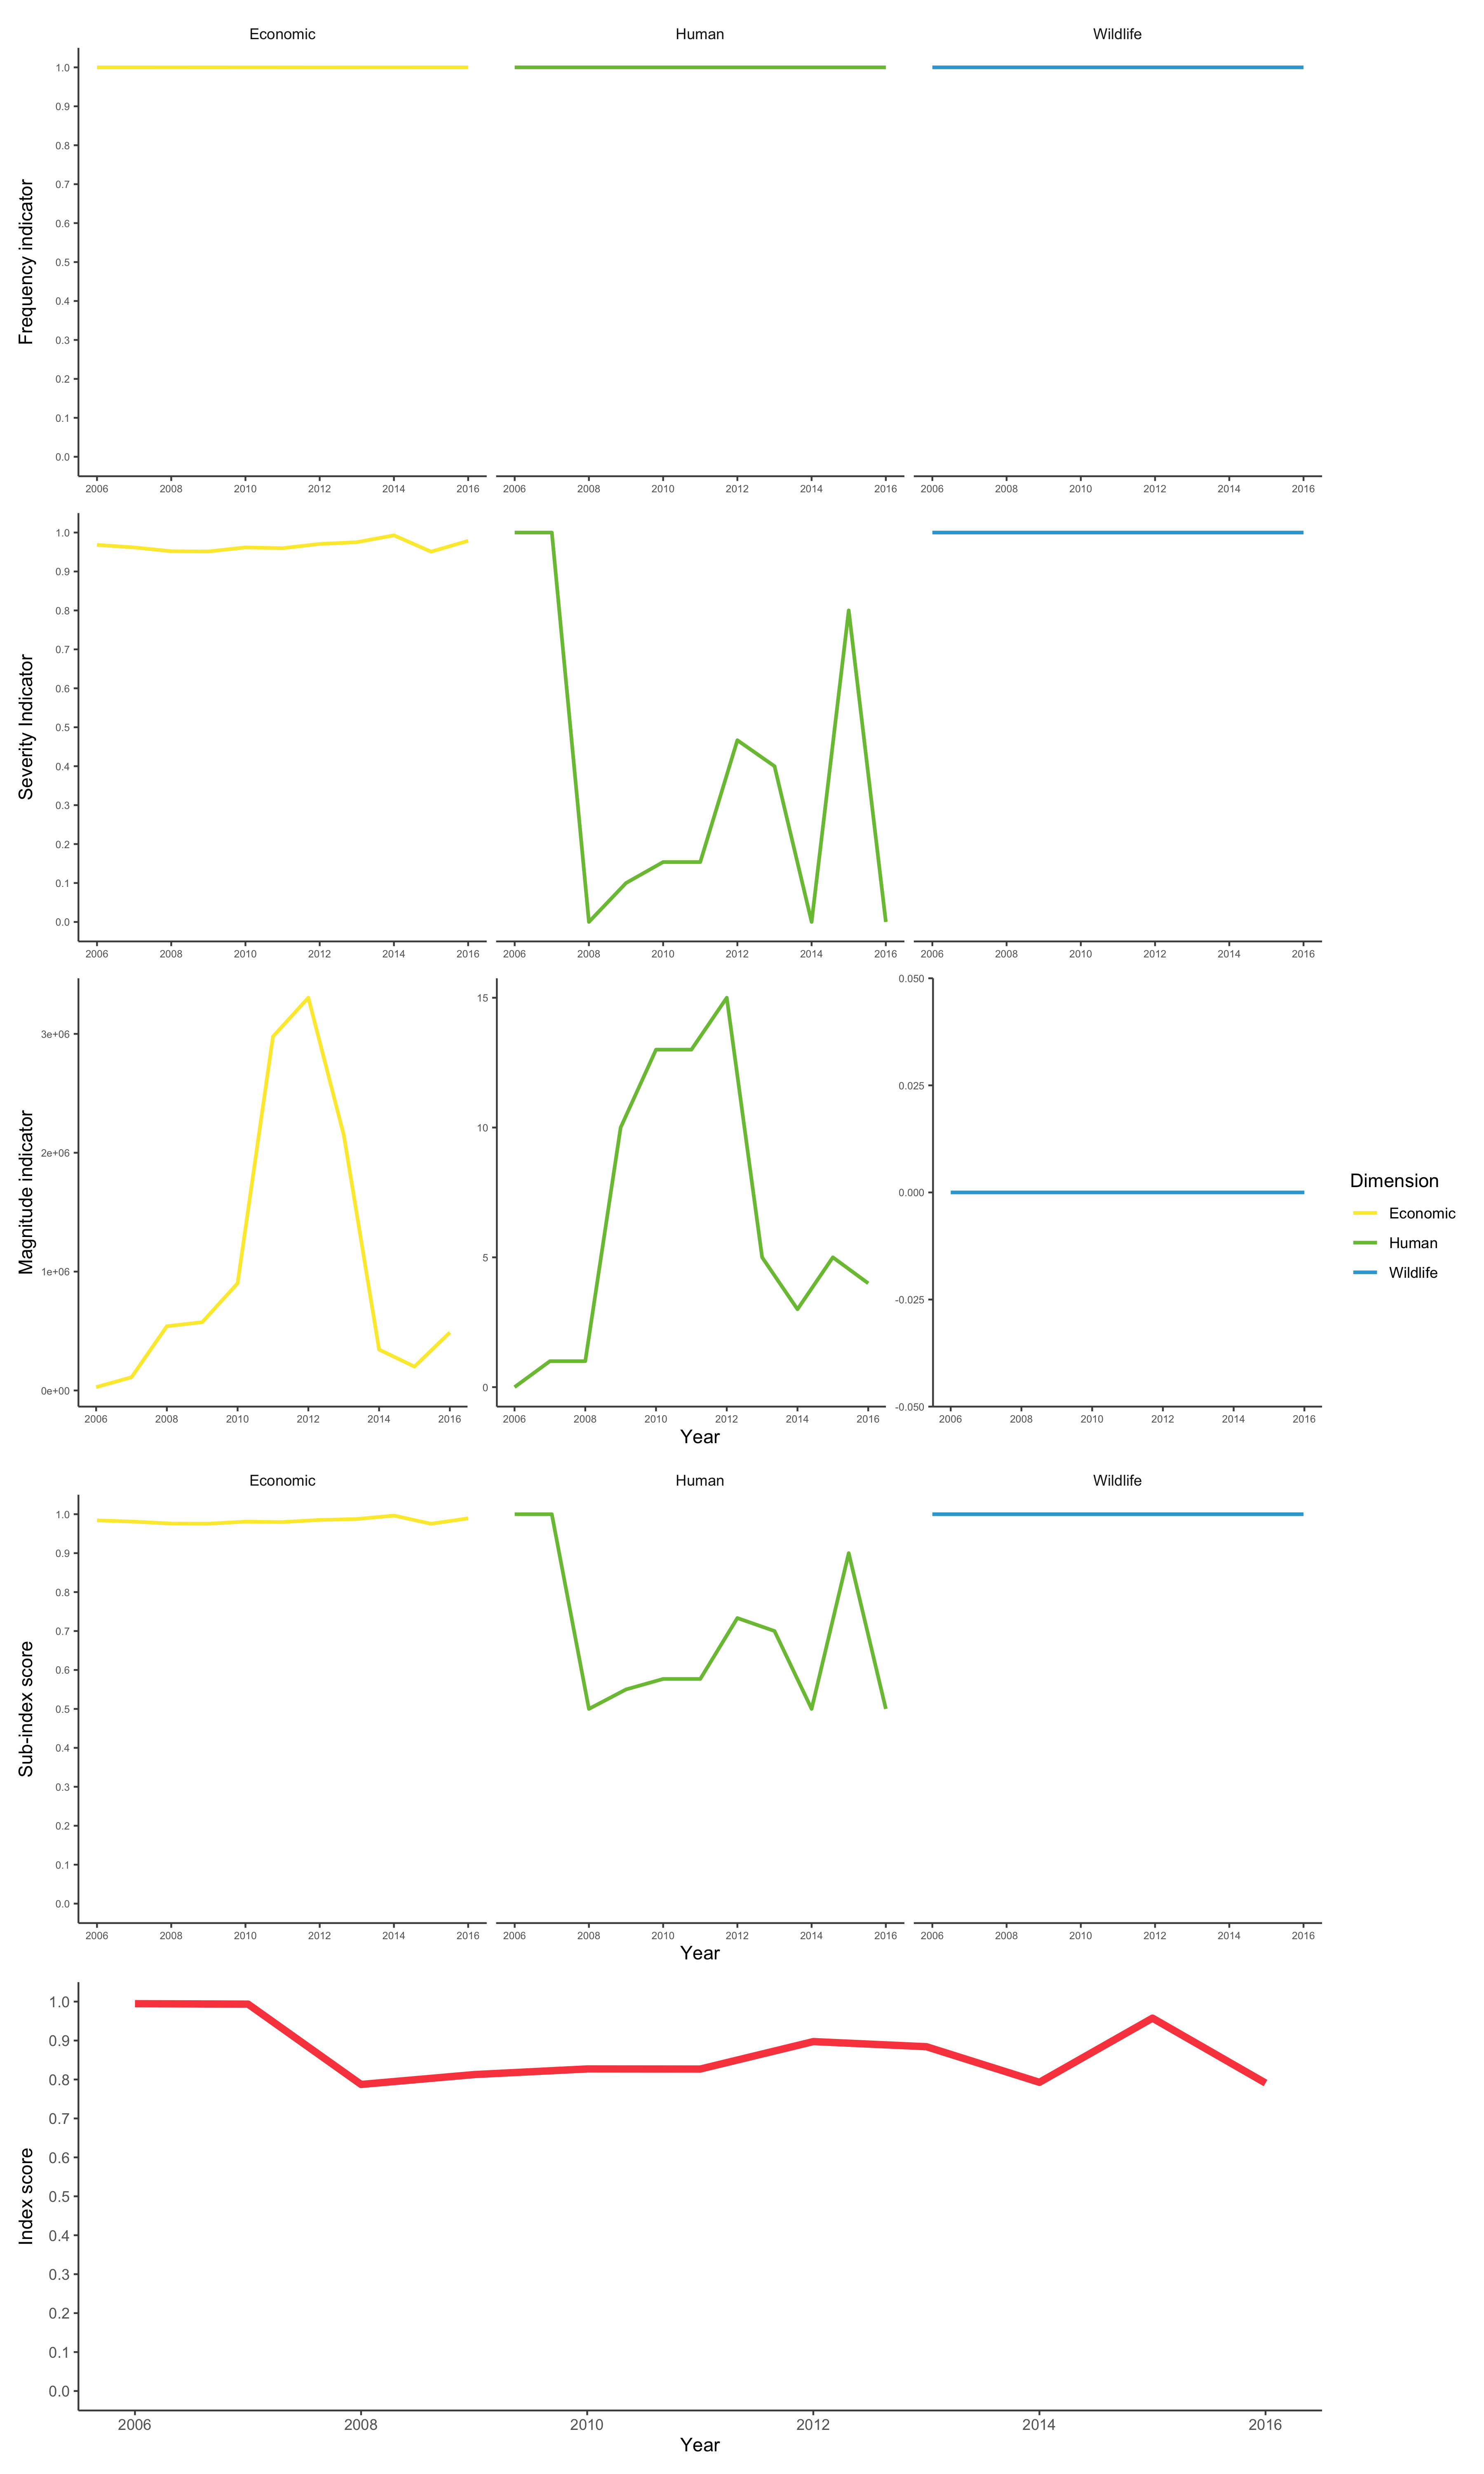
\includegraphics[width = 1\textwidth]{boar_all.png}
    \caption{Indicator suite for wild boar in Nepal.}
    \label{fig:boar}
\end{figure}

\end{document}


